\documentclass[11pt, titlepage]{report}

\usepackage{a4wide}
\usepackage[utf8]{inputenc}
\usepackage[czech]{babel}
\usepackage[pdftex]{graphicx}
\usepackage{indentfirst}
\usepackage{verbatim}
\usepackage{float}
\usepackage{amsmath}

\usepackage[top=2cm, left=2.75cm]{geometry}
\textwidth 16cm
\textheight 23cm
\renewcommand{\baselinestretch}{1.2}

\usepackage[
  pdftex,
  unicode,
  colorlinks,
  bookmarks,
  bookmarksnumbered,
  hypertexnames=false,
  breaklinks
]{hyperref}

\hypersetup{
  pdftitle={Eternity II},
  pdfauthor={Ondřej Garncarz},
  pdfsubject={Algoritmy pro řešení hlavolamu Eternity II},
  pdfkeywords={2, miliony, dolarů}
}

% \hypersetup{colorlinks=false}  % pro tisk

\floatstyle{ruled}
\newfloat{output}{htp}{lop}
\floatname{output}{Výpis}

\begin{document}

\sloppy

\begin{titlepage}
\centering
\begin{huge}
\begin{bfseries}
VŠB --- Technická univerzita Ostrava\\
Fakulta elektrotechniky a~informatiky\\
Katedra informatiky\\
\vfill
Algoritmy pro řešení hlavolamu Eternity~II\\
Algorithms for solving of Eternity~II puzzle\\
\vfill
\end{bfseries}
\end{huge}
2008/2009
\hfill
Ondřej Garncarz
\end{titlepage}


\chapter*{Prohlášení}
\thispagestyle{empty}

\noindent Prohlašuji, že jsem tuto bakalářskou práci vypracoval samostatně.

\noindent Uvedl jsem všechny literární prameny a~publikace, ze kterých jsem čerpal.

\vskip 5cm

\noindent Datum: 28.~dubna 2009
\hskip 0.4\linewidth
Ondřej Garncarz


\chapter*{Abstrakt a~klíčová slova}
\thispagestyle{empty}

\section*{Abstrakt}

\noindent Práce se zabývá pokusem nalézt různé přístupy k~řešení puzzle Eternity~II. Je vysvětlen princip puzzle a~rozebrána jeho složitost. Mezi přístupy k~řešení patří backtracking, simulované žíhání (simulated annealing), genetické algoritmy a~využití externích SAT solverů. Jednotlivé algoritmy jsou nejdříve představeny v~obecnosti~a následně ve vztahu k~Eternity~II. Všechny jsou reálně implementovány a~jejich efektivita je změřena a~zaznamenána. Tyto výsledky jsou na konci práce porovnány. Práce také obsahuje popis vyvinutého konvertoru pro formáty \textsc{Simplify} a~\textsc{Dimacs CNF}, jež se dá využít pro řešení libovolného problému pomocí určitých SAT solverů.

\section*{Abstract (in English)}

\noindent A~thesis is concerned with an~attempt to find different approaches to solve the~Eternity~II puzzle. The~principle of the~puzzle is described, as well as its complexity. The approaches include a~backtracking, a~simulated annealing, genetic algorithms and use of external SAT solvers. Each of them is presented at first in a~general way, then in the~Eternity II's matter. All algorithms are implemented and their efficiency has been measured and logged. The~results are compared at the~end. The~thesis also involves a~description of a~written \textsc{Simplify} and \textsc{Dimacs CNF} formats convertor which can be used for solving any problem by certain SAT solvers.

\section*{Klíčová slova}

\noindent Eternity~II, řešení hlavolamu, řešení těžkých problémů, NP-úplný, backtracking, simulované žíhání, genetické algoritmy, použití SAT solverů, Boolean satisfiability problem

\section*{Keywords (in English)}

\noindent Eternity~II, solving of puzzle, solving of difficult problems, NP-complete, backtracking, simulated annealing, genetic algorithms, use of SAT solvers, Boolean satisfiability problem


\setcounter{page}{0}
\tableofcontents


\chapter{Úvod}

Toto je práce zabývající se pokusem nalézt různé způsoby řešení pro puzzle Eternity~II a~jejich porovnání. Puzzle se skládá z~256 čtvercových dílků, kde každá strana dílku má určitý symbol a~poskládané puzzle musí mít na všech sousedících stranách stejné symboly. Puzzle je to tedy na první pohled velice jednoduché (má minimum pravidel) a~barevné --- ještě lákavější na něm však je možnost výhry dvou milionů dolarů. To však pouze v~případě, že se ho člověku podaří vyřešit jako prvnímu. Jelikož však problém koketuje s~NP-úplností, nebude to až tak jednoduché.

V Kapitole~\ref{ch:problem} tato práce pojedná o~problému samotném, čtenář jej pochopí a~pokud jej neosloví barevné obrázky, tak rozbor počtu možností či podkapitola o~NP-úplnosti určitě ano.

Kapitola~\ref{ch:program} naznačí, co všechno dokáže naimplementovaný program pro řešení tohoto puzzle. Přímé ovládání v~příkazové řádce však zatím zůstane zahaleno rouškou tajemství až do Kapitoly~\ref{ch:ovladani}.

Následující kapitoly nám již začnou představovat algoritmy řešení problému. Specifický algoritmus bude vždy popsán nejdříve v~obecnosti, bez návaznosti na Eternity~II. Popis ve vztahu k~puzzle a~náhled na implementaci budou obsahem následující podkapitoly. Poslední podkapitola je věnována výsledkům konkrétní implementace algoritmu --- tedy empirickému měření efektivity algoritmu.

Kapitola~\ref{ch:backtracking} je tedy věnována algoritmu backtrackingu, neboli řešení hrubou silou, avšak je využito souvislostí k~optimalizaci. Kapitola~\ref{ch:sa} se věnuje nedeterministickému simulovanému žíhání, inspirovanému procesem žíhání oceli. V~nedeterminističnosti pokračuje i~následující Kapitola~\ref{ch:ga}, popisující genetické algoritmy, inspirované evoluční biologií. Kapitola~\ref{ch:sat} se k~determinističnosti vrací, avšak pro řešení problému využijeme pomoci externích SAT solverů, řešičů logických formulí.

Výsledky všech měření jsou shrnuty v~Kapitole~\ref{ch:vysledky}, můžeme tedy porovnat jednotlivé algoritmy podle jejich efektivity a~přirozeně přikročit k~závěru.


\chapter{Problém}
\label{ch:problem}

Tato kapitola pojednává o~podstatě problému našeho puzzle --- jaká pro něj platí pravidla, jak tato pravidla určují počet možností řešení (Podkapitola~\ref{sec:problem-rozbor}) a~jak tento problém souvisí s~NP-úplností (Podkapitola~\ref{sec:problem-np}). 

Puzzle Eternity~II se skládá z~čtvercových dílků, kde každý dílek má na každé straně určitý symbol (viz Obrázek~\ref{jeden-dilek}). Cílem je poskládat dílky k~sobě tak, že dotýkající se strany dílků budou mít stejný symbol, přičemž výsledný tvar poskládaných dílků bude obdelník s~určenými rozměry ($N \times M$) a~šedý symbol bude právě na okrajích onoho obdelníku (viz Obrázek~\ref{plocha}).

\begin{figure}[ht]
\centering
\includegraphics[scale=0.5]{jeden-dilek.png}
\caption{Dílek skládanky}
\label{jeden-dilek}
\end{figure}

\begin{figure}[ht]
\centering
\includegraphics[scale=0.5]{6x6x6.png}
\caption{Poskládané puzzle pro 36 dílků s~využitím 6 možných symbolů (vymyšlený příklad)}
\label{plocha}
\end{figure}

\newpage V~implementovaném programu a~také v~této práci jsou strany dílků pojmenovávány podle světových stran (\emph{N} --- sever --- horní strana dílku, \emph{E} --- východ --- pravá strana, \emph{S} --- jih --- spodní strana, \emph{W} --- západ --- levá strana). Výsledný obdelníkový tvar s~rozměry $N \times M$ nazvěme hrací plochou. Pro oficiální Eternity~II puzzle platí $N = M = 16$, počet použitých symbolů je zřejmě 22 (toto je neověřená informace, distributor o~počtu symbolů nikde neinformuje). Kromě toho je ještě pro jeden konkrétní dílek určena jedna konkrétní pozice na hrací ploše. Velice důležité je, že dílky jsou rotovatelné, viz Obrázek~\ref{jeden-dilek-rot}.

\begin{figure}[ht]
\centering
\includegraphics[scale=0.5, angle=270]{jeden-dilek.png}
\caption{Rotovaný dílek \ref{jeden-dilek}}
\label{jeden-dilek-rot}
\end{figure}


\section{Rozbor problému}
\label{sec:problem-rozbor}

Zkusme si nejdříve nějak ohraničit složitost problému, ať víme, proti jak silnému nepříteli stojíme. Pro plochu o~rozměru $1 \times 1$ s~jedním celým šedým dílkem není o~čem přemýšlet, ale zvažme trochu rozumnější $2 \times 2$ s~4 dílky. I kdyby byl kromě šedé použit pouze jeden symbol, musíme již dílky rozmístit tak, aby byla právě ona šedá pouze na okrajích hrací plochy. Je jedno, na které pozici je který dílek, protože všechny mají stejný obsah, avšak záleží na rotacích --- totiž každý dílek může být rotován pouze jedním ze čtyřech způsobů ($0^\circ$, $90^\circ$, $180^\circ$, nebo $270^\circ$) --- to máme jinými slovy pro každý 1 správné nastavení ze 4 možných a~celkově pro plochu tedy 1 správné nastavení z~$4 \cdot 4 \cdot 4 \cdot 4 = 256$, což je překvapivě velké číslo.

Ono totiž nestačí možnosti nastavení sčítat, protože my daná správná nastavení jednotlivých dílků potřebujeme pro celou plochu současně, aby byla celá plocha vskutku správně nastavená (jinými slovy aby vyhovovala podmínkám). Podívejme se na dva obrázky níže --- jeden zachycuje správnou plochu, zde není moc řešit, soustřeďmě se na ten druhý --- tři dílky jsou rotovány správně (tedy jako 1 z~$4 \cdot 4 \cdot 4 = 64$ možností rotací této trojice), dílku vpravo nahoře zbývají 4 možnosti, ale je uplatněna nevhodná.

\begin{figure}[ht]
\centering
\begin{minipage}[b]{0.4\linewidth}
\centering
\includegraphics[scale=0.5]{2x2x1-spravna.png}
\caption{Správná plocha}
\end{minipage}
\begin{minipage}[b]{0.4\linewidth}
\centering
\includegraphics[scale=0.5]{2x2x1-chybna.png}
\caption{Chybná plocha}
\end{minipage}
\end{figure}

Situace se stává komplexnější a~také komplikovanější, pokud na stejně velké ploše použijeme symbolů více --- vezměme nyní rovnou čtyři. Kromě šedé na okrajích budeme muset již pohlídat i~párování symbolů. Začněme od levého horního rohu --– můžeme dosadit libovolný dílek (každý je pro takto velkou plochu rohový) --- musíme ho však donastavit (zrotovat) pouze jednou ze čtyřech možností. Na druhé pozici (tedy vpravo nahoře) již ovšem nemůže být jakýkoliv dílek --– daný dílek musí mít na západní straně symbol shodný s~východním symbolem souseda, navíc při dodržení správné rotace! Máme tedy 4~možnosti pro natočení a~vybíráme ze 3 dílků. Správně řečeno je to ale spíše obráceně --- vybíráme ze 3~dílků a~\emph{u~každého} máme navíc 4 možnosti pro natočení --- protože máme k~dispozici celkem 4~symboly, bude každý dílek odlišný od kteréhokoliv jiného (i~kdybychom rotovali), a~tedy máme pro druhou pozici $3 \cdot 4 = 12$ možností nastavení (aneb jak již bude definitivně na ploše dílek vypadat).

\begin{figure}[ht]
\centering
\includegraphics[scale=0.5]{2x2x4.png}
\caption{Plocha $2 \times 2$ se 4 symboly}
\end{figure}

Pro třetí pozici (vlevo dole) vybíráme již jen ze 2 dílků --- tudíž je zde $2 \cdot 4 = 8$ zbývajících možných nastavení (nebo-li pokud na první dvě pozice dáme libovolné dva dílky, zde je již dát nemůžeme --- takto omezujeme možnosti). Pro poslední pozici --- vpravo dole --- nám zbude vždy již jen jeden dílek, u~něj tedy budeme uvažovat stejně jako u prvního jenom ony 4 možnosti rotace.

A~nakonec pro celou plochu tedy platí: $4 \cdot 12 \cdot 8 \cdot 4 = 1536$ možností nastavení, z nichž pouze jedno jediné je správné. (Ono ve skutečnosti je více možností nastavení --- pokud bychom brali první pozici taktéž jako volnou a~nechali do ni dosadit všechny 4 dílky. Avšak toto je zcela zbytečné, protože pokud na začátku zvolíme jeden rohový dílek pro jeden roh jako fixní, jistě je to správné nastavení, protože případy, kdy by byl v~jiných rozích, jsou pouze rotací celé plochy.)

Nyní si zkusíme provést takovýto rozbor pro plochu se vším všudy (tedy i~nerohovými okrajovými dílky a~vnitřními dílky), a~to především obecně. Bude proto vhodné si jednotlivé pozice na ploše nějak označit, aby bylo pochopení rychlejší.

\begin{figure}[ht]
\centering
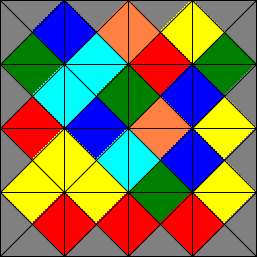
\includegraphics[scale=0.5]{4x4x6.png}
\caption{Plocha $4 \times 4$ se 6 symboly}
\end{figure}

\newpage
\begin{table}[ht]
\centering
\begin{tabular}{|c|c|c|c|}
\hline
$R_1$ & $O_1$ & $O_2$ & $R_2$ \\ \hline
$O_8$ & $V_1$ & $V_2$ & $O_3$ \\ \hline
$O_7$ & $V_4$ & $V_3$ & $O_4$ \\ \hline
$R_4$ & $O_6$ & $O_5$ & $R_3$ \\
\hline
\end{tabular}
\caption{Označení pozic na ploše $4 \times 4$}
\end{table}

\begin{description}
\item[$R_1$] 1 dílek, 4 rotace (Rotace budou všude 4, každý dílek lze totiž tolikrát natočit, my nemůžeme vědět, které natočení bude vhodné do plochy. Proto v~tomto seznamu nebudou rotace dále uvádeny.)
\item[$R_2$] 3 dílky (zbývající rohové dílky)
\item[$R_3$] 2 dílky (zbývající rohové dílky)
\item[$R_4$] 1 dílek (poslední rohový dílek)
\item[$O_1$] 8 dílků (okrajové dílky)
\item[$O_2$] 7 dílků (zbývající okrajové dílky)
\item[\vdots]
\item[$O_7$] 2 dílky (zbývající okrajové dílky)
\item[$O_8$] 1 dílek (poslední okrajový dílek)
\item[$V_1$] 4 dílky (vnitřní dílky)
\item[$V_2$] 3 dílky (zbývající vnitřní dílky)
\item[$V_3$] 2 dílky (zbývající vnitřní dílky)
\item[$V_4$] 1 dílek (poslední vnitřní dílek)
\end{description}

Ze seznamu výše lze intuitivně vyvodit toto: rotace můžeme vyčlenit mimo, možností rotací pro celou plochu je $4^{N \cdot M}$, kde $N \times M$ je velikost plochy. Pro uspořádání rohových dílků je vždy $1 \cdot 3 \cdot 2 \cdot 1 = 6$ možností.

Okrajových dílků je pode velikosti plochy $(N - 2) + (M - 2) + (N - 2) + (M - 2) = 2N + 2M - 8 = 2 \cdot (N + M - 4)$. A možností pro uspořádání těchto dílků je $(2 \cdot (N + M - 4))!$.

U vnitřních dílků je situace podobná --- jejich počet je $(N - 2) \cdot (M - 2)$, možností pro uspořádání je $((N - 2) \cdot (M - 2))!$.

Celkově máme tedy pro uspořádání dílků na ploše $6 \cdot (2(N + M - 4))! \cdot ((N - 2) \cdot (M - 2))!$ možností. Pokud chceme mít finální vzoreček, tak připočteme (resp. přinásobíme) ještě možnosti rotací, tudíž výsledek je $6 \cdot (2 \cdot (N + M - 4))! \cdot ((N - 2) \cdot (M - 2))! \cdot 4^{N \cdot M}$. Následuje tabulka pro některé konkrétní velikosti plochy, kolik to tak může být (vypočítáno v~programu \textsc{QtOctave 0.7.2}). Jde vidět, že počty možností jsou velice vysoké, ale toto ještě nemusí nutně znamenat, že problém je těžké vyřešit (cesta k~řešení může být v~každém případě lehká).

\begin{table}[ht]
\centering
\begin{tabular}{|c|c|}
\hline
\textbf{velikost plochy ($N \times M$)} & \textbf{možností nastavení} \\ \hline
$2 \times 2$ & $1 536$ \\ \hline
$2 \times 3$ & $49 152$ \\ \hline
$3 \times 3$ & $37 748 736$ \\ \hline
$4 \times 4$ & $2,493 7 \cdot 10^{16}$ \\ \hline
$5 \times 5$ & $1,174 2 \cdot 10^{30}$ \\ \hline
$6 \times 6$ & $1,240 4 \cdot 10^{49}$ \\ \hline
$7 \times 7$ & $7,175 6 \cdot 10^{73}$ \\ \hline
$8 \times 8$ & $4,712 3 \cdot 10^{104}$ \\ \hline
$9 \times 9$ & $6,505 1 \cdot 10^{141}$ \\ \hline
$10 \times 10$ & $3,219 1 \cdot 10^{185}$ \\ \hline
$11 \times 11$ & $9,144 5 \cdot 10^{235}$ \\ \hline
$12 \times 12$ & $2,272 2 \cdot 10^{293}$ \\
\hline
\end{tabular}
\caption{Počty možností nastavení plochy pro různé velikosti}
\label{tabulka-moznosti}
\end{table}


\section{NP-úplnost problému}
\label{sec:problem-np}

Ve článku \cite{np-dukaz} byla dokázána NP-úplnost problému téměř shodného s~Eternity~II. Proto je tohoto důkazu nyní využito.

Problém je \emph{NP-úplný}, pokud je \emph{NP-těžký} a~zároveň náleží do třídy \emph{NP}. Problém Eternity~II zjevně do třídy NP náleží --- polynomiální nedeterministický algoritmus by mohl snadno nedeterministicky ,,uhodnout`` rozmístění dílků a~poté ověřit, zda je toto rozmístění korektní. NP-těžkost problému je definována jako možnost polynomiálně převést jakýkoliv problém z~třídy NP na daný problém (podle \cite[str.~261]{np-skripta}). Proto dokáže-li náš problém zakódovat již ověřený NP-těžký problém, je náš problém taktéž NP-těžký.

Pro případ Eternity~II použijme \emph{3-partition problem}, který je NP-úplný, tudíž NP-těžký a~jeho podstata je následující (podle \cite{np-3par-wiki}):

\begin{itemize}
\item Vstupem je množina přirozených čísel $S$, která obsahuje $n = 3 \cdot m$ prvků, kde $m$ je přirozené číslo.
\item Otázka zní, jaké je rozdělení $S$ do $m$ trojic tak, aby každý prvek náležel právě jedné trojici a~aby si součty všech trojic byly rovny.
\item Takovéto sumy jsou rovny $\Sigma = 3 \cdot B$ a~problém zůstává NP-úplným i~při omezení hodnot prvků na interval mezi $\frac{B}{4}$ a~$\frac{B}{2}$ (což se nám bude hodit).
\end{itemize}

Proto pokud vezmeme v~potaz plochu jako na Obrázku~\ref{np-plocha}, kde každý z~užitých symbolů (kromě šedé na okraji a~modré a~zelené) je použit právě pro jeden pár dílků, tedy daná plocha je pro tento případ fixní, neboli nejde jinak rozestavit, tak poté můžeme na dosud nevyplněnou černou oblast plochy pohlížet jako na místo pro zakódování 3-partition problému.

\begin{figure}
\centering
\includegraphics[scale=0.5]{np-plocha.png}
\caption{Plocha s~černou dírou pro dokázání NP-těžkosti}
\label{np-plocha}
\end{figure}

Jednotlivé prvky z~množiny $S$ nechť jsou zakódovány podle své hodnoty tak, že hodnota určuje nový unikátní symbol na ploše a~existuje tolik dílků s~daným symbolem, že jejich horizontálním spojením vznikne řádek dílků dlouhý stejně jako je hodnota prvku. Příklad takového řádku lze vidět na Obrázku~\ref{np-radek}.

\begin{figure}
\centering
\includegraphics[scale=0.5]{np-radek.png}
\caption{Řádková formace dílků pro prvek z~množiny $S$}
\label{np-radek}
\end{figure}

Tyto řádky musí mít na horizontalním okraji modrou barvu a~na vertikálním zelenou. To poté zaručuje, že dílky budou moci býti užity pouze dohromady ve formě těchto \emph{řádků} a~budou moci býti do černé oblasti plochy vkládány pouze horizontálně.\footnote{Pokus vložit je jiným způsobem by vedl k~porušení pravidel puzzle ohledně shodných sousedících symbolů.} Problém tedy bude zároveň problémem Eternity~II a~zároveň problémem uspořádání \emph{řádků} tak, aby byla vyplněna černá oblast plochy, jejíž šířka odpovídá konstantní sumě trojice $\Sigma$ a~jejíž výška odpovídá počtu trojic $m$, což je 3-partition problém.\footnote{Na jeden celý černý řádek se mohou vlézt pouze právě tři \emph{řádky} prvků, to díky omezení hodnot prvků na interval od $\frac{B}{4}$ do $\frac{B}{2}$.}

3-partition problém je tedy převoditelný do problému Eternity~II, a~problém Eternity~II je tedy NP-těžký. Jeho příslušnost k~třídě NP ho řadí navíc i~mezi NP-úplné problémy.


\chapter{Program}
\label{ch:program}

Tato kapitola ve stručnosti ukazuje možnosti implementovaného programu, konkrétní ovládání je popsáno až v~Kapitole~\ref{ch:ovladani}.

Jelikož program vyžaduje jako vstup zadání určité hrací plochy (neboli dílky, které budou k~dispozici), obsahuje program generátor náhodných ploch, aby uživatel nemusel vytvářet své vlastní nebo si snad dokonce kupovat originál. Pro vytvářené plochy je nutné zadat, jakých budou rozměrů a~z~kolika možností symbolů budou moci čerpat.

První implementovaný způsob řešení je backtracking a~lze u~něj ovlivnit způsob procházení plochy, pořadí dílků při jejich vybírání a~také lze aktivovat způsob řešení tzv. netrpělivým backtrackingem, kdy program dává po určité době přednost náhodnému rozházení dílků a~startu odznova před dokončením aktuálního prohledávání.

Druhým implementovaným způsobem je simulované žíhání (Simulated Annealing) --- tento způsob nemá volitelné parametry.

Třetí implementovaný algoritmus je pseudogenetický algoritmus, taktéž bez parametrů.

Čtvrtý je genetický algoritmus --- zde lze ovlivnit způsob kódování jedinců, váhu kladnou na dodržování pravidel, nebo naopak na shodnost nových dílků s~dílky ze zadání a~pravděpodobnost mutací.

Posledním, pátým, implementovaným postupem je využití externích SAT solverů. Lze ovlivnit, zda bude vytvořená logická formule znegovaná, či nikoli.

Pro kompletní ošetření režie běhu externích SAT solverů, stejně jako grafické zobrazování hracích ploch, lze využít implementovaných pomocných skriptů, resp. přídavného programu zobrazovače.


\chapter{Backtracking}
\label{ch:backtracking}

Tato kapitola pojednává o~řešení problému backtrackingem, prohledáváním všech možností do hloubky. Podkapitola~\ref{sec:bck-obecne} popisuje tento princip v~obecnosti, bez návaznosti na puzzle Eternity~II --- tomuto je věnována Podkapitola~\ref{sec:bck-et}. Podkapitola~\ref{sec:bck-vysl} se věnuje výsledkům backtrackingu dosažených implementovaným programem.

\section{Backtracking v~obecnosti}
\label{sec:bck-obecne}

Každý NP-úplný problém, resp. problém, ve kterém hledáme správné řešení v~rámci všech možností, tedy v~prostoru všech možných kombinací nastavení určitého \emph{světa}\footnote{Uvažujme svět jako ,,prostor`` problému --- umožňuje všechny jeho vlasnosti a~projevy.}, lze intuitivně řešit zkoušením oněch kombinací. Tedy procházíme všechna možná nastavení světa a~u~každého kontrolujeme, zda-li jsme nenašli nastavení, které vyhovuje podmínkám cíle. Tomuto způsobu se říká řešení \emph{hrubou silou} nebo též řešení \emph{backtrackingem}.

Konkrétněji postupujeme takto: nalezneme první \emph{bod světa}, který tvoří jeho různorodost. Tedy takový bod, jehož stav ovlivňuje stav celého světa. Jestliže není jisté, který bod ve světě je pro tento účel první, může být kterýkoliv, avšak je nutné při následujícím výběru bodů dodržet pravidlo, že každý bod měnící stav světa bude brán v potaz. Tomuto prvnímu bodu přiřadíme první možnost \emph{nastavení}, první \emph{stav}. Opět platí, že pokud neexistuje přirozené pořadí stavů pro bod, je možné vybírat stavy náhodně, avšak každý musí být využit.

Při nastaveném prvním, resp. $n$-tém, bodu světa přejdeme k stavu druhému, resp. $n + 1$. U~něj postupujeme stejně jako u~bodu $n$-tého (zůstaneme nyní již u~obecného pořadí) --- vybereme tedy první možnost jeho stavu a~zanoříme se do stavu $n + 2$. Takto postupujeme, dokud nepřiřadíme nějaký konkrétní stav i~poslednímu rozhodujícímu bodu světa. V~tomto okamžiku již tedy máme sestaven celý konkrétní svět, jeho první možnost. Prověříme jej, jestli vyhovuje podmínkám cílového světa. V případě pozitivního vyhodnocení je celý problém vyřešen.

Pokud je vyhodnocení negativní, budeme se vracet nazpátek. Přiřadíme tedy poslednímu bodu následující možný stav. Pokud již byly všechny jeho stavy vyčerpány, vracíme se nazpátek k~předposlednímu bodu, mu přiřadíme následující možný stav a~u~posledního bodu přiřadíme první možný stav (protože pro dané nastavení předchozích bodů je toto první možností). Obecně se vracíme nazpátek tak dlouho, dokud jsou u konkrétních bodů všechny stavy již vypotřebovány. Jestliže se vracíme nazpátek a~dokonce i~první bod má již vypotřebovány všechny stavy, znamená to, že jsme prošli všemi stavy světa, ale žádný při kontrole nevyhovoval podmínkám cíle, tudíž že řešení neexistuje.

Tento způsob hledání řešení využívá \emph{rekurze} --- to je ono zanořování, při kterém na každé úrovni pracujeme pouze s~jedním bodem a~provádíme jej tak dlouho, dokud jsou nějaké body k~dispozici. Tomuto způsobu využití rekurze se konkrétně říká \emph{prohledávání do hloubky}.

Paměťová složitost tohoto algoritmu je polynomiální (často lineární --- využijeme právě tolik paměti, kolik bodů má náš svět). Časová složitost je exponenciální --- v~zanořování u~každého bodu provedeme tolik kroků, kolik má možných stavů, a~navíc se v~každém tomto kroku zanoříme hlouběji, kde provádíme to samé. Každý konkrétní stav světa projdeme a~zkontrolujeme právě jednou.

\section{Backtracking v~Eternity~II}
\label{sec:bck-et}

Backtracking se v~implementaci nalézá především v~souborech \texttt{src/backtracking.*} (\emph{především} proto, že se odvolává i~na jiné funkce --- ty pracující s~dílky a~plochou, viz \texttt{src/cards.*} a~\texttt{src/area.*}).

\emph{Světem} je pro nás hrací plocha. \emph{Body světa}, které určují jeho rozmanitost a~výsledné vlasnosti, jsou jednotlivé čtverečky na ploše. \emph{Nastavením} těchto bodů jsou dílky umístěné na nich, včetně jejich rotace. Takto obsáhneme jakoukoliv možnost řešení a~toto je tedy také podstatou implementace backtrackingu v~Eternity~II.

Nejdříve je načtena plocha zadání do programu. K~uložení je využito trojrozměrné pole integerů \texttt{area}, kde první index určuje řádek plochy, druhý sloupec a třetí (světovou) stranu dílku. Hodnotou je použitý symbol. Zároveň v~případě použivání zafixovaných dílků jsou tyto dílky zkopírovány do pole \texttt{area\_fixed\_card}, toto však není příliš důležité. Tento způsob zpracování plochy je stejný pro všechny postupy.

Následně jsou z~\texttt{area} získány informace o~výběru dílků, ze kterého budeme čerpat při sestavování cílové plochy. Věc se má takto: pokud máme obsazená pouze určitá políčka na ploše dílky a~vybereme si další políčko pro dosazení vhodného dílku, které je již některými dílky obklopeno, tak máme omezenou možnost výběru vhodných dílků. Nejen faktem, že již použité dílky využít nemůžeme, ale také strany dílku, které se budou dotýkat již dosazených dílků, musí obsahovat symbol, který se bude se sousedem párovat. Je-li toto omezení využito, přinese velikou úsporu času, protože zabraňuje rozvíjení rekurze v~případech nesmyslných ploch --- tedy takových, které k~cíli určitě nevedou.

Proto existuje čtyřrozměrné pole \texttt{symbol\_cards}, kde jednotlivé indexy udávají v~následujícím pořadí: spodní (jižní) symbol souseda nahoře, levý (západní) symbol souseda napravo, horní (severní) symbol souseda dole a pravý (východní) symbol souseda nalevo. Jinými slovy udávají, čemu musí symboly daného dílku vyhovovat, přičemž je nutno uvažovat speciální hodnotou i~dosud nedosazený symbol (tedy volnost výběru aktuálního dílku) a~nesmíme opomenout ani šedý symbol. Hodnotami pole jsou struktury \texttt{t\_symbol\_card}, které obsahují tyto informace: reálný vzor dílku, počet volných dílků s~daným vzorem a~odkaz na další strukturu, odpovídající stejnému obecnému vzoru, určenému indexy pole. Reálný vzor dílku se od vzoru určenému indexy pole liší tím, že všechny jeho symboly musí být určité (ne hodnota pro nedosazený symbol) --- to proto, že zde se již odvoláváme na konkrétní dílky. Toto také vysvětluje existenci odkazu na další strukturu --- jednomu vzoru určenému indexy pole, ve kterém se nachází neurčený symbol, může odpovídat více vzorů konkrétních. Počet volných dílků přináší další úsporu času --- jestliže na určitou pozici plochy dosadíme konkrétní dílek \emph{A} nebo \emph{B}, přičemž oba mají stejné vzory, je jedno --- ale zkoušet obojí zvlášť v~backtrackingu při rekurzivním zanořování by přidalo určitý čas navíc, viz Log~\ref{log2}.

Pole \texttt{symbol\_cards} je tedy doplněno během procházení všech dílků plochy, přičemž každý konkrétní dílek je do něj vložena $4 \times$ --- každá rotace zvlášť --- bez tohoto bychom nebyli schopni následně pole využít rozumným způsobem. Je zbytečné při samotném backtrackingu neustále dokola rotovat ty samé dílky, když tuto operaci můžeme vykonat již nyní a~to pouze jednou (tedy další úspora času). Při tomto je ale třeba mít na mysli, že počet volných dílků daného vzoru je tedy hodnotou společnou čtyřem konkrétním rotovaným vzorům, a~proto je tato hodnota uložena v~paměti jen jednou a~struktura vzoru dílku se na ni pouze odvolává ukazatelem.

Následně je v~programu nutno ujasnit, jakým způsobem budeme plochu procházet --- jakým způsobem budeme hledat ony \emph{body světa}. Existuje proto jednorozměrné pole \texttt{steps}, kde hodnotami jsou struktury udávající řádek a sloupec plochy. Index pole udává pořadí. V~implementaci máme na výběr z řádkového, šikmého a~spirálovitého setřídění políček plochy. V~každém setřídění jsou však privilegována nejdříve rohová políčka a~poté ostatní okrajová --- to kvůli faktu, že dílky do těchto políček se vybírají z~těch obsahujících dva, resp. jeden šedý symbol. Když totiž poté při backtrackingu nejdříve vytvoříme okraj plochy, budou již všechny dílky obsahující šedé symboly použity a~nebudou zkoušeny uvnitř plochy, kde podle pravidel být nemohou, a dosáhneme tak další úspory času.

Samotný backtracking probíhá následovně:
\begin{enumerate}
\item Pokud jsme se dostali zatím nejdále (tedy nejvíce dosažených dílků), uložíme plochu do souboru \texttt{area\_backtrack\_temp.area}.
\item V~případě \emph{netrpělivého backtrackingu}\footnote{Takovýto backtracking neprohledává všechny možnosti --- dává přednost po uplynutí časového (či krokového) limitu náhodnému promíchání vstupních prvků ve snaze přiblížit ideální vyhledávací větev co nejblíže začátku prohledávání.} ověříme, zda-li míra trpělivosti již nepřetekla a~nemáme začít odznova, nebo-li jestli máme náhodně rozházet dílky a~začít s~backtrackingem od první pozice.
\item Jinak podle fáze backtrackingu poznáme, jestli nemáme pracovat s~fixním dílkem (případně s~kterým) --- ten dosadíme a~pro každou jeho rotaci se zanořujeme hlouběji do rekurze.
\item Jinak otestujeme, zda-li se nám již nepodařilo všechny dílky dosadit --- pokud ano, tak máme vyhráno, backtracking totiž neustále dodržoval pravidla, výsledná plocha je tudíž korektní. Taková plocha je uložena do souboru \texttt{area\_backtrack\_result.area} a~backtracking je ukončen.
\item Jinak podle pozice, pro kterou zrovna dosazujeme dílky, zjistíme vzor, kterému musí dosazované dílky vyhovovat. Jej využijeme jako čtyřrozměrný index pro nalezení prvního vhodného dílku v~předem připraveném poli \texttt{symbol\_cards}. Každý volný dílek postupně obsadíme na danou pozici a~sestoupíme hlouběji v rekurzi. Je zde možnost využít náhodného pořadí vybírání dílků ze~\texttt{symbol\_cards} (tedy že se pro daný obecný vzor na různých pozicích nebudou zkoušet dílky vždy ve stejném pořadí).
\end{enumerate}

\section{Výsledky backtrackingu pro Eternity~II}
\label{sec:bck-vysl}

Experimentálně se jako nejefektivnější jeví procházet plochu spirálovitě. Využití netrpělivého backtrackingu či náhodného vybírání dílků se jako efektivní nejeví. Existují celkem tři statistiky experimentů pro backtracking --- Log~\ref{log1}, Log~\ref{log2} a~Log~\ref{log7} --- logy jsou obsaženy v~příloze této práce a~kopírují obsahy souborů \texttt{results/*.html}, ty však navíc obsahují odkazy na jak vstupní, tak originální plochy, pro které byly experimenty prováděny.

Podle výsledků je program například schopen vyřešit plochu $4 \times 4 \times 4$ i~$6 \times 6 \times 6$ \emph{na odenterování}, ale oficiální plocha $16 \times 16$ je beznadějná, jelikož již v~řešení ploch $8 \times 8 \times 8$ a~$9 \times 9 \times 9$ existuje řádově podstatný časový rozdíl --- pár sekund versus několik minut až hodina, a to navíc plocha $10 \times 10 \times 10$ nebyla vyřešena ani během 24~hodin.


\chapter{Simulated Annealing}
\label{ch:sa}

Tato kapitola pojednává o~principu řešení prohledávacích problémů pomocí Simulated Annealing, nedeterministického algoritmu inspirovaného průmyslovým procesem žíhání oceli. Podkapitola~\ref{sec:sa-obecne} vysvětluje princip v~obecnosti, Podkapitola~\ref{sec:sa-et} je věnována implementaci pro problém Eternity~II. Podkapitola~\ref{sec:sa-vysl} shrnuje výsledky experimentů s~touto implementací.

\section{Simulated Annealing v~obecnosti}
\label{sec:sa-obecne}

Simulated Annealing (\emph{simulované žíhání}) simuluje proces kontrolovaného žíhání oceli, kdy je usilováno o~snížení vnitřní energie oceli, kterážto reflektuje stav jejího strukturálního uspořádání, nebo-li kvalitu oceli. Na začátku procesu je ocel rozehřáta na vysokou teplotu, přičemž čím vyšší teplota je, tím více se struktura oceli mění (tepelná energie je zužitkována pohybem atomů). Následně je teplota snižována, čímž se pohyby atomů zpomalují a~struktura oceli se ustaluje. Jelikož atomy se přirozeně přesouvají do pozic s~nižší vnitřní energií, nebo-li dostávají se z~pozic \emph{semknutějších} do pozic \emph{volnějších}, čehož je jim dopřáno právě onou potřebnou vysokou energií, celková vnitřní energie tělesa oceli klesá. Na konci procesu je tedy ocel učiněna kvalitnější, avšak nemusí to být skutečné optimum, neboť kroky restrukturilizace vedou ve většině případů ke stavům příbuzným aktuálnímu stavu a zároveň kvalitnějším, nikoliv však nutně nejkvalitnějším. Proces žíhání oceli tedy není časově omezen, v~případě nespokojenosti s~kvalitou se dá teplota opakovaně zvyšovat a opět nechávat klesat, což zvyšuje pravděpodobnost, že se kvalita oceli zvedne, vnitřní energie sníží. Výsledek procesu tudíž není nutně optimální, a~deterministicky předpověditelný již vůbec ne.

V~informatickém pojetí je \emph{ocelí} stav světa, známý již z~backtrackingu. \emph{Atomy oceli} jsou prvky světa. \emph{Vnitřní energie} je obrácenou hodnotou kvality světa, čili blíží se k~nule tím více, čím blíže je nastavení světa podmínkám světa cílového. Tato energie se dá určit s~přihlédnutím ke kvalitám jednotlivých prvků světa, atomů oceli. Na začátku procesu simulovaného žíhání je náhodně zvolen první stav, resp. k~žíhání je připravena ocel nevalné kvality. Dokud není dosažena požadovaná kvalita nebo např. není překročen maximální přípustný počet kroků žíhání, je \emph{ocel žíhána}. K~tomu dochází určením náhodného stavu světa, který je příbuzný aktuálnímu stavu. Jestliže je jeho kvalita, jeho vnitřní energie, menší, tudíž výhodnější, než aktuální, stav světa se skutečně na takovýto změní. Pokud je nová kvalita horší, nemusí být takovýto stav světa nutně zahozen, je možné do něj přejít, ale jen s~určitou pravděpodobností, vypočítanou na základě staré kvality, nové kvality a~například teploty nebo kroku žíhání.

Vylepšením může být pamatování si zatím nejlepšího stavu, protože vracením se do stavů s~horší kvalitou se sice můžeme vyhýbat stagnace v~lokálních optimech, ale zároveň se nám již lepší stav nemusí podařit najít.

Paměťová složitost algoritmu je lineární --- paměťi budeme potřebovat tolik, jak je náš svět veliký. Časová určitelná není, neboť algoritmus není deterministický --- díky využívání náhody při sestavování nových stavů a~rozhodování o~přijetí méně kvalitnějších stavů. (Časová) efektivnost je tedy hodnocena experimentálně empiricky.

Simulated Annealing bylo nastudováno podle \cite{sa-wiki} a~\cite{sa-papers}.

\section{Simulated Annealing v~Eternity~II}
\label{sec:sa-et}

Jádro implementace je umístěno v~souborech \texttt{src/annealing.*}. Po načtení plochy zadání \texttt{area.area} jakožto \emph{oceli} je spočítána její \emph{vnitřní energie} a~tato plocha a~energie jsou uloženy jako zatím nejlepší a~také poslední. Určování energie funguje takto: pro každý dílek jsou spočteny penalizační body za porušování pravidel, kde je po jednom bodu za neshodu se sousedem či nešedý symbol na neokrajové pozici. Celková energie plochy je sumou jednotlivých penalizací.

Při práci s~fixními dílky dochází při nedodržení každé jednotlivé pozice k~penalizaci ve formě zdvounásobení celkové energie.

Dokud je vnitřní energie větší než nula, nebo-li v~ploše existují spory proti pravidlům, a~je tedy co zlepšovat, protože jsme zatím nedosáhli cílové plochy, konáme následující:

\begin{enumerate}
\item Získáme plochu sousední/blízkou aktuální. Toho je dosaženo buďto náhodnou rotací náhodného dílku nebo prohozením dvou náhodných sousedících dílků.
\item Nové ploše/oceli je spočtena energie.
\item Pokud je nová energie zatím nejlepší (čili nejnižší), je přesun do nového stavu zachován a~nová plocha a~energie jsou uloženy jako nejlepší.
\item Pokud není nová energie tak nízká, je přesun do nového stavu zachován podle pozitivního výsledku náhody určené nerovnicí $e^{\frac{e_{s} - e_{n}}{t}} > r$, kde $e_{s}$ je stará energie, $e_{n}$ nová energie, $t$ aktuální teplota a~$r$ náhodné reálné číslo v~intervalu $<0,1>$. Teplota je určena podle kroku žíhání jako $\frac{10^{7}}{(k \mod{10^{7}}) + 1}$, kde $k$ je krok, čili v~periodicky se opakujících klesáních nepřímé úměrnosti od $10^{7}$ k~$1$. Konstanty i~celého způsobu výpočtu teploty bylo dosaženo experimenty, jejich výsledky jsou zachyceny v~Logu~\ref{log3}.
\end{enumerate}

V~průběhu algoritmu jsou doposud nejlepší plochy ukládány jako \texttt{area\_anneal\_temp.area}, na konci je cílová plocha uložena do \texttt{area\_anneal\_result.area}.

\section{Výsledky Simulated Annealing pro Eternity~II}
\label{sec:sa-vysl}

Statistiky experimentů se simulovaným žíháním jsou zachyceny v~Logu~\ref{log3} a~Logu~\ref{log6}. V~implementaci \emph{SA} lze v~podstatě ovlivnit tři věci --- výběr nejbližšího stavu, výpočet energie a~určování teploty. První dvě věci byly zvoleny intuitivně, nebyl jsem si vědom pro daný problém principiálně odlišného postupu. Nejefektivnější výpočet teploty byl určen experimenty, kdy například pro plochu $4 \times 4 \times 4$ byla výsledná plocha nalezena průměrně během půl minuty až minuty --- viz Log~\ref{log3}.

Podle Logu~\ref{log6} je však tato velikost plochy maximální přípustná pro praktické řešení --- program nebyl schopen vyřešit plochu o~velikosti $5 \times 5 \times 5$ ani během 24~hodin.


\chapter{Genetické algoritmy}
\label{ch:ga}

Tato kapitola popisuje genetické algoritmy, nedeterministické algoritmy inspirované evoluční teorií. Podkapitola~\ref{sec:ga-obecne} představí princip v~obecnosti, bez návaznosti na naše puzzle. Pro něj však vznikly rovnou dvě implementace, proto jsou popsány odděleně. První implementaci --- ,,pseudogenetický algoritmus`` popisuje Podkapitola~\ref{sec:ga-pseudo}, její výsledky Podkapitola~\ref{sec:ga-pseudo-vysl}. Implementaci více se blížící principu genetických algoritmů pak popisuje Podkapitola~\ref{sec:ga-ga}, jejím výsledkům se věnuje Podkapitola~\ref{sec:ga-ga-vysl}.

\section{Genetické algoritmy v~obecnosti}
\label{sec:ga-obecne}

V~přírodě se dá pro algoritmy hledat inspirace i~v~organické oblasti, jako je tomu například u~genetických algoritmů inspirovaných evoluční biologií. Informaticky se dají \emph{GA} popsat následovně:

Mějme \emph{populaci} jedinců, kde každý \emph{jedinec} je svým způsobem souhrnem určitých vlastností --- \emph{genů}. Populace obsahuje v~určitý čas určitý počet jedinců, toto značíme generací. Jedinou činností, která se opakovaně odehrává, je rozmnožování --- tvoření potomstva, další generace. Je to dáno účelem --- jedinci pomocí svých genů představují, resp. kódují, způsob řešení určitého problému, tato řešení mohou být různě kvalitní a my chceme nalézt to nejlepší řešení, pokud možno to nejlepší možné. Nechceme tedy, aby jedinci něco konali, pouze hledáme toho nejlepšího, protože on samotný je řešením problému, aniž by o~tom vlastně věděl.

Populace nechť je tedy nazírána jako souhrn vícero možných řešení problému, který chceme opakovanou procedurou --- \emph{rozmnožováním} --- dostat do takového stavu, aby v~přijatelném čase obsahoval jedince, který nám bude zcela vyhovovat, či se alespoň k~našim požadavkům přijatelně přiblíží. Procedura probíhá takto:

\begin{enumerate}
\item Spočítáme \emph{kvality} jedinců na základě jejich genů. Pokud je některá kvalita dostačující, pokračování nemá smysl.
\item Vybereme jedince, kteří postoupí do další generace nebo se stanou rodiči jedinců následující generace. Tato akce se nazývá \emph{selekce}.
\item Následuje \emph{křížení} --- geny postupivších jedinců jsou smíchány, aby takto vytvořily nové jedince, kteří buďto automaticky postoupí do nové generace, nebo postoupí kvalitnější z~rodičů, nebo potomků --- záleží na implementaci, může také záviset na náhodě, protože obecně vzato náhoda hraje v~ne zcela deterministických algoritmech, jakými GA jsou, velikou roli, ne však vždy pozitivní --- záleží na vyladění jednotlivých náhod a~postupů, ale toto je již otázkou implementace.
\item Pro neopakování neustále stejných či velice podobných genů, v~důsledku tedy i~jedinců a~populací, a~možné obohacení slouží \emph{mutace}, která mění náhodné geny či jejich části náhodných jedinců.
\end{enumerate}

Při selekci se dá vybírat podle kvality ty nejlepší jedince nebo třeba vybráním vždy toho kvalitnějšího ze dvou náhodných. Existují i~propracovanější metody (co do složitosti), například \emph{vážená ruleta}, kdy dochází k~náhodným losováním z~jedinců, kde pravděpodobnost jedince ke zvolení je tím větší, čím víc je kvalitní vůči ostatním.

Křížení jedinci mohou mít geny například polovinu po prvním rodiči, polovinu po druhém nebo více náhodile, případně i~z~více rodičů.

Obecný princip GA je nastudován podle \cite{ga-poli} a~\cite{ga-dipl}.

\section{Pseudogenetický algoritmus v~Eternity~II}
\label{sec:ga-pseudo}

První implementace ,,genetických algoritmů`` je genetickými algoritmy spíše jen inspirovaná, její jádro se nachází v souborech \texttt{src/pseudognt.*}. Při inicializaci dojde k~načtení plochy zadání a~spočítání četnosti dílků podle jejich symbolů (a~to pro všechny rotace dílků) --- v~čtyřrozměrném integerovém poli typu \texttt{cards\_count\_t} je podle indexů udávajích symbol na dané straně (v~klasickém pořadí \emph{N}--\emph{E}--\emph{S}--\emph{W}) uložena ona četnost pro dílky mající daný vzor.

Následně je vygenerována nová, náhodná plocha a~je jí taktéž spočtena četnost dílků, čehož je bezprostředně využito při určování kvality oné nové plochy. Každému jednotlivému dílku je určena kvalita, jako součet kvality za \emph{původ} a~za \emph{vhodnost}\footnote{Kvalita za původ značí shodnost se zadanými dílky, kvalita za vhodnost vystihuje dodržování pravidel puzzle (stejné symboly na sousedních stranách).} na dané pozici (tato je však v~implementaci zbytečná, protože plocha v~každém okamžiku vyhovuje pravidlům, a~proto je reálně uvažována pouze kvalita za původ). Pokud dílek nové plochy není obsažen v~rozházené ploše zadání, což se zjistí jednoduše porovnáním příslušných hodnot v~polích typu \texttt{cards\_count\_t}, je jeho kvalita za původ nulová. Maximální (1,0) kvalitu má v~případě, že dílek mající daný vzor je v~zadání také obsažen, a~to nejvýše v~počtu ekvivalentnímu počtu z~nové plochy. Pokud je v~nynější ploše dílků s~daným vzorem více než v~originále, není to zrovna žádaný stav, proto bude kvalita původu rovna $\frac{p_{p}}{p_{n}}$, kde $p_{p}$ je původní počet a~$p_{n}$ nový počet. Celková kvalita plochy je průměrem kvalit jednotlivých dílků, pohybuje se v~rozmezí $<0, 1>$.

\newpage Při práci s~fixními dílky dochází při nedodržení každé jednotlivé pozice k~penalizaci ve formě jednak vynulování kvality dílku na dané pozici a~jednak snížení hodnoty celkové kvality na polovinu.

Dokud není kvalita rovna 1,0, pokoušíme se populaci \emph{vylepšit} --- pokud pro každou dílek převáží náhoda nad kvalitou, pokusíme se daný dílek \emph{vylepšit} (proto je tedy větší pravděpodobnost změny u~méně kvalitních dílků). K~vylepšování dochází pro každou stranu dílku zvlášť --- u~okrajových stran je šedá barva nutností (pokud nechceme porušit pravidla), jinak záleží na náhodě --- pokud opět náhoda převáží nad kvalitou\footnote{Neboli ze stejného intervalu, jako má kvalita, je vylosováno náhodné číslo a~následně je toto číslo porovnáno s~kvalitou.}, nyní ovšem sousedního dílku, jsou změněny dotýkající se strany na náhodný symbol, jinak je symbol zkopírován od onoho sousedního dílku (tedy v nynější implementaci, kdy neustále dodržujeme pravidla, totéž co nezměněn). Ke kontrole kvality sousedních dílků dochází z~důvodu nevole měnit kvalitní dílky.

Po pokusu vylepšit populaci (která v~této implementaci znamená hrací plochu, kde jedinci jsou dílky, kteří však zastupují řešení problému vždy pouze z části, není to plně terminologie \emph{GA}) aktualizujeme kvality a~v~případě zatím nejvyšší kvality je aktuální plocha vypsána a~uložena do souboru \texttt{area\_pseudognt\_temp.area}. Takto pokračujeme, dokud nedosáhneme cíle --- plochy, která jednak splňuje pravidla hry (což je v~této implementaci automatické) a~zároveň vychází plně z~dílků zadání. Takováto plocha je uložena do \texttt{area\_pseudognt\_result.area}.

Implementace navíc obsahuje kontrolu \emph{stagnace} --- pokud se kvalita plochy po určitý počet kroků pohybuje v~malém rozmezí, zřejmě jsme uvázli na mrtvém bodě, proto je ploše mírně pomoženo --- určitý zlomek dílků je změněn na náhodné dílky (přičemž jsou změněny vždy i~sousední symboly, aby nedošlo k porušení pravidel).

\section{Výsledky pseudogenetického algoritmu pro Eternity~II}
\label{sec:ga-pseudo-vysl}

Na základě provedených měření, která jsou zdokumentována v~Logu~\ref{log5}, lze vyčíst, že pseudogenetický algoritmus je prakticky rychlý pro plochy do velikosti $4 \times 4 \times 4$ včetně --- řešení je nalezeno v~řádu sekund. Poté dochází k~výraznému nárůstu potřebného času, kdy nalezení řešení pro plochu $5 \times 5 \times 5$ je otázkou hodin, až k~neznámému času přesahujícímu jeden den potřebnému pro plochu $6 \times 6 \times 6$.

\section{Genetický algoritmus v~Eternity~II}
\label{sec:ga-ga}

Co do objemu zdrojových kódů a~počtu různých operací je o~dost větší implementace opravdového \emph{GA}, umístěná v~\texttt{src/genetics.*}. Inicializace probíhá stejně --- je načtena plocha zadání a~spočtena četnost dílků podle jejich symbolů, stejným způsobem. Nyní však nebudeme pracovat s~hrací plochou, nebudeme upravovat ji, ale budeme pracovat s~již opravdovou \emph{populací} obsahující \emph{jedince}, jež budou pouze kódovat obsah hrací plochy --- proto existuje typ \texttt{t\_string}, který je polem boolean hodnot a~kóduje hrací plochu, obecně by mohl kódovat jakýkoliv problém. Typ \texttt{t\_population} je polem \texttt{t\_string}ů a~reprezentuje populaci (určitý počet jedinců) v~určitém čase, tedy \emph{generaci}.

\emph{Kódování} je implementováno dvěma rozlišnými způsoby, mezi kterými si argumentem při spuštění můžeme vybrat. Prvním je kódování plochy jako symbolů --- \texttt{t\_string} obsahuje postupně pro každou pozici na ploše (čtením řádku zleva doprava a pak přechodem na řádek další) pro všechny strany (opět v klasickém pořadí \emph{N}--\emph{E}--\emph{S}--\emph{W}) bitové zakódování (pramenící z boolean hodnot) symbolu. Jelikož takto mohou být zakódovány i~nepřípustné hodnoty symbolů, je možno využít, a~v~implementaci je využito, při dekódování modulo pro korekci hodnoty.

Druhá možnost je kódování pozic s~rotacemi. Zde je postupně pro každou pozici na ploše bitová hodnota pozice dílku z~plochy zadání (v~1D formátu --- čili v~podstatě ne pozice, ale pořadí --- jež je ale snadno přepočitatelné na pozici) a~bitová hodnota rotace onoho dílku ze zadání. Nepřípustné hodnoty jsou opět korigovány na přípustné.

Tyto různé možnosti kódování tedy nakládají odlišnými způsoby s~pamětí a~potřebují jí rozdílné množství --- toto je bráno v~potaz a~na začátku běhu algoritmu jsou vypočteny maximální bitové délky jednotlivých typů hodnot, aby pak při samotných dekódovacích výpočtech byl šetřen čas.

Po inicializaci program pokračuje vytvořením první generace, kde každý bit každého jedince populace je náhodou určen jako \texttt{true}, nebo \texttt{false}. Následně je v~populaci nalezen nejlepší řetězec --- nejlepší jedinec, a~to tak, že každého jedince dekódujeme na hrací plochu a~ji ohodnotíme, způsobem velmi podobným ohodnocování z~implementace pseudogenetického algoritmu --- nejprve spočítáme četnost dílků podle jejich symbolů, poté pro každý dílek na ploše určujeme kvalitu původu (zcela stejným způsobem) a~kvalitu sousednosti --- čím více dílek vyhovuje okolním symbolů, tím lépe. Celková kvalita dílku v~rozmezí $<0, 1>$ je dána součtem těchto dvou kvalit, přičemž můžeme procentuálně měnit jejich vzájemnou důležitost (například 60~\% pro původ a~40~\% pro sousednost). Celková kvalita plochy je pak průměrem kvalit jednotlivých dílků.

Při práci s~fixními dílky dochází při nedodržení každé jednotlivé pozice k~penalizaci ve formě jednak vynulování kvality dílku na dané pozici a~jednak snížení hodnoty celkové kvality na polovinu.

Dokud není kvalita nejlepšího řetězce --- totiž nejlepší plochy --- rovna 1,0, nedosáhli jsme cíle a~pokračujeme v~běhu genetického algoritmu. Nejdříve populaci \emph{reprodukujeme} --- pomocí vážené rulety vybereme jedince nové generace. Existuje pole reálných čísel \texttt{roulette}, kde jsou při průchodu jedinců uloženy jejich intervaly na ruletě, počítáno podle jejich kvalit, a~nakonec je ruleta přepočtena na reálný interval $<0, 1>$. Poté je tolikrát, kolik je jedinců (jejich počet je konstantní), losováno náhodné číslo v~rozmezí $<0, 1>$ a~šťastný jedinec na daném intervalu, nalezený pomocí půlení intervalů, je zkopírován do nové generace (ne vzat, protože na něj může náhoda ukázat vícekrát).

V~dalším kroku populaci \emph{křížíme} --- dokud to jde, vybíráme náhodně dva staré zatím však nevybrané jedince k~možnému rodičovství. Na jejich místo v~poli populace nakopírujeme jedince z~kraje pole a~velikost pole virtuálně snížíme (tímto je dosaženo vybírání dosud nevybraných). Poté losujeme. Pokud náhoda padne na rodičovství (tuto pravděpodobnost lze nastavit argumentem programu), jedince zkřížíme --- a~to buďto ne-nutně stejně velkými ,,polovinami`` (čili jim v~podstatě onu druhou ,,polovinu`` prohodíme) nebo náhodně po bitech. Způsob je opět nastavitelný při startu. Pokud náhoda na rodičovství neukáže, jedinci do nové generace postupují netknutí. Nakonec, jestliže je počet jedinců v~populaci lichý, posledního zbývajícího jedince do nové generace jenom překopírujeme.

Posledním krokem je \emph{mutace} --- každému jednotlivci u~každého bitu náhodně určíme, zda-li jej znegujeme, či ponecháme. Pravděpodobnost je opět určitelná při startu, obyčejně je využíváno téměř nulové hodnoty.

Pokud je v~průběhu \emph{GA} nalezen lepší jedinec než zatím nejlepší, je vypsán a~plocha, kterou reprezentuje, je uložena do souboru \texttt{area\_genetics\_temp.area}. Pokud je dosaženo cíle, je cílová plocha uložena také do souboru \texttt{area\_genetics\_result.area}.

Tato implementace je nastudována podle \cite{ga-dipl}, jež mě jako učebnice genetických algoritmů zaujala svojí jednoduchostí a~názorností.

\section{Výsledky genetického algoritmu pro Eternity~II}
\label{sec:ga-ga-vysl}

Genetický algoritmus v~Eternity~II nevykazuje žádnou efektivitu. Jak lze vidět v~\cite{ga-dipl}, způsob zakódování problému je nadmíru důležitý --- pro kódování čísel lze využít \emph{Grayova kódu}, kdy se kódování dvou sousedních čísel (pro určitý problém) liší pouze v~jednom bitu, kódování tedy svým způsobem zachovává blízkost/vzdálenost stavů. V~problému Eternity~II však nebyl objeven, ani tedy využit, podobně sofistikovaný způsob kódování --- toto může vysvětlovat prakticky nulovou šanci algoritmu dostat se do cílového stavu.


\chapter{SAT}
\label{ch:sat}

Tato kapitola popisuje řešení problému pomocí využití externích SAT solverů. V~Podkapitole~\ref{sec:sat-obecne} bude vysvětleno, co to vůbec SAT solver je a~jak takový způsob řešení může v~obecnosti fungovat. Podkapitola~\ref{sec:sat-et} popisuje implementace principu pro puzzle Eternity~II, pro přehlednost je rozdělena do dvou podpodkapitol --- Podpodkapitola~\ref{subsec:sat-et-simplify} pojednává o~využití formátu \textsc{Simplify} a~Pododkapitola~\ref{subsec:sat-et-cnf} o~využití formátu \textsc{Dimacs CNF}. Poslední Podkapitola~\ref{sec:sat-vysl} zmiňuje výsledky dosažené těmito implementacemi.

\section{SAT v~obecnosti}
\label{sec:sat-obecne}

Jelikož cílem informatiky je věci člověku usňadnovat a~prostředkem tohoto je kromě jiného dosahování čím dál tím větší univerzálnosti, vznikl i~trend vyvíjení programů řešící složité problémy uživatelů, jež jsou zapsatelné ve formě logické formule, kdy splnění problému je dosaženo skrze nalezení hodnot proměnných formule, pro které je formule pravdivá. Tomuto se v~angličtině říká \emph{boolean satisfiability problem}, odtud také zkrácený název SAT\footnote{Podle \cite[str. 182]{np-skripta} je SAT problém definován následovně: vstupem je booleovská formule v~konjunktivní normální formě, otázkou zda-li je daná formule splnitelná (tj. existuje pravdivostní ohodnocení proměnných, při kterém je formule pravdivá).}.

Z~pohledu uživatele majícího problém je jedinou jeho starostí nalézt zakódování problému do logické formule a~po vyřešení dekódování výsledku. Interní fungování \emph{SAT solverů} --- oněch programů řešících problém --- je věcí vývoje, kdy mohou být uplatňovány postupy jako backtracking, heuristiky nebo genetické algoritmy či cokoliv myslitelného, vše je zaměřeno pouze na optimální výkon, protože složitost řešení logických formulí spadá do \emph{NP}. Rozvoji používaných algoritmů napomáhají i~různé SAT soutěže.

Jedním z~možných formátů formule je, sice prefixový, ale lidsky snadno čitelný, zápis programu \textsc{Simplify}, kde můžeme zapsat jakkoliv strukturovanou formuli, která sestává z~proměnných, operátorů logického součinu, součtu a~negace a~závorek pro upravení priorit a~zanořování. Ukázka je ve Výpisu~\ref{simplify-in}, whitespacy jsou programem ignorovány.

\begin{output}
\begin{verbatim}
(AND
    prvni
    (OR
        druha
        (NOT treti_promenna)
    )
)
\end{verbatim}
\caption{Vstupní formát pro \textsc{Simplify}}
\label{simplify-in}
\end{output}

\newpage \textsc{Simplify} ale hledá protipříklad, proto pokud chceme najít opravdové řešení naší formule, musíme ji celou znegovat, jak je tomu ve Výpisu~\ref{simplify-in-negace}, na nějž nám dá program řešení ve formátu příkladu výčtu proměnných, které při současné kladné hodnotě ruší tautologii formule, Výpis~\ref{simplify-out-right}. Pokud je výsledek formátu podle Výpisu~\ref{simplify-out-false}, je formule tautologií, tedy v~případě užití negace celé naší původně zamýšlené formule jako vstupu se jedná o~opak --- naše formule není nikdy řešitelná, je kontradikcí.

\begin{output}
\begin{verbatim}
(NOT
    (AND
        prvni
        (OR
            druha
            (NOT treti_promenna)
        )
    )
)
\end{verbatim}
\caption{Upravený vstup programu \textsc{Simplify}}
\label{simplify-in-negace}
\end{output}

\begin{output}
\begin{verbatim}
Counterexample:
  context:
    (AND
      druha
      prvni
    )

1: Invalid.
\end{verbatim}
\caption{Výstup programu \textsc{Simplify}}
\label{simplify-out-right}
\end{output}

\begin{output}
\begin{verbatim}
1: Valid.
\end{verbatim}
\caption{Jiný výstup programu \textsc{Simplify}}
\label{simplify-out-false}
\end{output}

\newpage Za zmínku stojí fakt, že program \textsc{Simplify} formálně spadá spíše pod skupinu \emph{automated theorem proving}, která se věnuje dokazování matematických vět, my jej však zde uvažujeme spíše jen jako \emph{SAT solver}.

Druhý z~možných formátů využívá specializovanější struktury logické formule --- konjunktivní normální formy (\emph{CNF}, conjunctive normal form), která je ve tvaru konjunkcí klauzulí, které jsou disjunkcemi literálů, které jsou buďto proměnnými, nebo jejich negacemi. Jako standard v~SAT se pro toto vyvinul formát nazvaný \textsc{Dimacs CNF}, který však již pro člověka tolik intuitivně čitelný jako \textsc{Simplify} formát není --- zápis problému ekvivalentnímu tomu ve Výpisu~\ref{simplify-in} je ve Výpisu~\ref{cnf-in}. Tento formát byl společně s~formátem téměř ekvivalentím se \textsc{Simplify} nastudován podle \cite{sat-formats}.

\begin{output}
\begin{verbatim}
p cnf 6 9
2 -1 0
3 -1 0
-2 -3 1 0
-4 3 0
-5 3 0
4 5 -3 0
-6 -5 0
6 5 0
1 0
\end{verbatim}
\caption{Vstup ve formátu \textsc{Dimacs CNF}}
\label{cnf-in}
\end{output}

Formální první řádek \texttt{p cnf <počet proměnných> <počet klauzulí>} je povinný, předmětné jsou však až následující, kde je jeden řádek pro jednu klauzuli. Řádek pak obsahuje literály klauzule, jež jsou v případě pozitivní hodnoty přímo proměnnými, jinak negacemi proměnných. Proměnné nemají jména, ale jsou číslovány. Whitespacy jsou ignorovány, řádek klauzule ukončuje \texttt{0}, která není číslem proměnné. Některé programy mají problémy při interpretaci delších řádků bez enterů.

Výstupní formát udává splnitelnost formule a~případně výčet hodnot proměnných, při kterém je formule splnitelná. Pozitivní číslo proměnné znamená pravdivou hodnotu, negativní opačnou. Výčet je ukončen nulou. Například pro problém zapsaný ve Výpisu~\ref{cnf-in} je výsledek ve Výpisu~\ref{cnf-out}.

\begin{output}
\begin{verbatim}
s SATISFIABLE
v 1 2 3 -4 5 -6 0
\end{verbatim}
\caption{Výstup ve formátu \textsc{Dimacs CNF}}
\label{cnf-out}
\end{output}

Obecně není efektivnost SAT solverů nikterak zaručena --- například některé mohou brzo nalézt správné řešení, ale zjištění kontradikce není v~přijatelném čase vůbec zaručena. Při \emph{šťastném} rozestavění proměnných a~klauzulí může být naopak i~velice těžký problém vyřešen velmi rychle. Obecně je možný jakýkoliv průběh.

\section{SAT v~Eternity~II}
\label{sec:sat-et}

Implementace řešení problému tímto způsobem je rozdělena do dvou částí. Hlavní program \texttt{eternity} umožňuje vytvoření zápisu v~\textsc{Simplify} formátu a~také následné dekódování výsledku do hrací plochy --- zdrojové kódy jsou v~\texttt{src/sat.*} a~\texttt{src/unsat.*}. Druhou částí jsou překladače SAT$\rightarrow$CNF a~(výsledku) CNF$\rightarrow$SAT, \texttt{bin/sat2cnf.py} a~\texttt{bin/cnf2sat.py}.

\subsection{Simplify}
\label{subsec:sat-et-simplify}

K~popisu vztahů na ploše stačí tři základní typy proměnných (kurzivá značí proměnnou --- místo daného slova či slovního spojení dojde k~dosazení požadované hodnoty):

\begin{description}
\item[card\_position\_$card\_nr$\_\_$x$\_$y$] dílek na pozici --- pro každou kombinaci čísla dílku (\emph{card\_nr}) a~pozice (\emph{x} a~\emph{y}) existuje proměnná říkající, zda-li se daný dílek nachází na dané pozici
\item[card\_rotation\_$card\_nr$\_$rot$] rotace dílku --- pro každou kombinaci čísla dílku (\emph{card\_nr}) a~rotace (\emph{rot}) existuje proměnná říkající, zda-li je daný dílek rotován danou rotací
\item[area\_symbol\_$x$\_$y$\_\_$side$\_$symbol$] symbol na straně pozice --- pro každou kombinaci pozice (\emph{x} a~\emph{y}), strany (\emph{side}) a~symbolu (\emph{symbol}) existuje proměnná říkající, zda-li se na dané straně dané pozice nachází daný symbol
\end{description}

Je nutné ohlídat, aby každý dílek byl na ploše právě jednou a~aby žádné dva nebyly na stejné pozici. Disjunkce \texttt{card\_position} proměnných pro každou pozici jednoho určitého dílku zaručuje, že dílek bude někde na ploše.\footnote{U~fixních dílků je uplatněna pouze jediná platná pozice.} Konjunkce těchto disjunkcí zaručuje výskyt všech dílků někde na ploše. Konjunkce dosavadního s podmínkou pro maximálně jeden dílek na každé jednotlivé pozici zajistí kompletní využití plochy. Maximálně jeden dílek na pozici je určen rekurzivním omezováním možnosti použití dílku buďto pouze z~první, nebo pouze z~druhé poloviny možných dílků (proměnných).\footnote{Jsou vzaty všechny proměnné a~rozděleny na dvě poloviny --- následně je vytvořeno pravidlo, že platit může některý prvek buďto pouze z~první, nebo pouze z~druhé poloviny. Dokud to je možno, stejný postup je uplatněn rekurzivně i~na dané poloviny.}

Dále je nutno připojit (konjunkcí --- defaultně vždy konjunkcí, aby platilo vše, co má) podmínku pro právě jednu rotaci pro každý dílek. Toho je dosaženo opět disjunkcí všech rotací jednoho dílku ($\Rightarrow$ dílek bude rotována) a~dále omezením platnosti maximálně jedné ze dvojice proměnných rotace dílku, přičemž toto je určeno pro každou možnou dvojici. Rozklad možných proměnných půlením intervalů a~omezování platnosti pro maximálně jednu polovinu není nutné použít, protože u~rotace jsou pouze čtyři možnosti.

Poté, co máme hotová pravidla pro obsazení plochy dílky, zajistíme pravidla pro obsahy jednotlivých políček, jednotlivé symboly. Jde o~implikaci s podstatou $\texttt{card\_position} \wedge \texttt{card\_rotation} \rightarrow \texttt{area\_symbol}$, po úpravě (\textsc{Simplify} totiž neumí přímo implikaci) $\neg (\texttt{card\_position} \wedge \texttt{card\_rotation}) \vee \texttt{area\_symbol}$. Toto pravidlo musí být tedy uplatněno pro všechny možné kombinace.\footnote{Opět u~fixních dílků netřeba uvažovat jiné než fixní souřadnice.}

Následně již zbývá pouze připojit podmínky pro dodržení pravidel hry. Jsou dvojího typu: okrajové šedé symboly a~symboly sousedící, vnitřní. Pro \texttt{area\_symbol} na okrajové pozici musí platit šedý symbol, proměnné daného typu pro ostatní symboly musí být nepravdivé, negované. Na vnitřních pozicích právě naopak nesmí být šedý symbol, ale právě jeden ze zbývajících. Toto je podmíněno stejným rekurzivním dělením jako u~\texttt{card\_position} ($\Rightarrow$ maximálně jeden symbol), společně však s~minulou podmínkou pro kompletní zaplnění plochy implikuje právě jede symbol. Shodnost symbolů se sousedními není třeba prosazovat, protože \texttt{area\_symbol} je při kódování problému do formule ve skutečnosti přepočítáváno pouze na jižní a~východní stranu dílku --- je-li tedy použita strana severní nebo západní, využije se místo ní sousedící strany sousedícího dílku.

Tyto podmínky ve své celistvosti určují problém Eternity~II pro zadané dílky a~uloženy do souboru \texttt{sat.txt}, je možno nad nimi spustit externí program \textsc{Simplify}. Celou režii řešení má v~tomto případě pod sebou skript \texttt{bin/simplify.sh}. Po vyřešení, v~případě vyřešení, je možno dekódovat SAT výsledek umístěný v~souboru \texttt{sat\_result.txt} do zápisu hrací plochy \texttt{area\_sat\_result.area} --- každý řádek vstupního souboru je v~případě nevýskytu negace (\texttt{NOT} na začátku) dosazen do vzoru pro \texttt{area\_symbol\_$x$\_$y$\_\_$side$\_$symbol$} --- v~případě úspěchu je na danou stranu dané pozice plochy umístěn daný symbol. Na sousedící stranu sousedícího dílku také, kvůli úsporné neexistenci \emph{NORTH} a~\emph{WEST} stran pro \texttt{area\_symbol}. Jinými slovy podle výsledku SAT solvingu zjistíme, jaké symboly kterých stran kterých pozic plochy jsou pravdivé.

\subsection{CNF}
\label{subsec:sat-et-cnf}

Pro použití externích řešících programů, které pracují pouze s~CNF formulemi, byl vyvinut \textsc{Python}ovský skript volatelný jako \texttt{sat2cnf.py <input\_file> <output\_file>}, který formuli umístěnou ve vstupním souboru v~\textsc{Simplify} formátu převede do výstupního souboru s~formátem \textsc{Dimacs CNF}. Skript si nejdříve během procházení vstupního souboru rekurzivně vytvoří stromovou strukturu instancí vlastní třídy \texttt{Node}, jež reflektuje větvení formule podle operátorů (s~výjimkou operátorů $\neg$) --- instance obsahuje buďto užitý operátor, označení uzlu a~pole potomků (operandů), nebo pouze přímo proměnné v~případě listů, přičemž názvy uzlů a~proměnných jsou překládány do unikátních čísel (protože \textsc{Dimacs CNF} pracuje s~takovýmto značením). Překladová tabulka je ukládána do souboru \texttt{cnf\_translation.txt}, kde na lichém řádku je překladové číslo a~na následujícím sudém řádku originální značení, přičemž originální značení uzlů je tvořeno řetězcem \texttt{tmp} a~jejich překladovým číslem, protože žádné původní značení ve skutečnosti ani nemají.

Výjimka negace je rozšířením umožňujícím redukci počtu uzlů, implikuje tedy snadnější a~rychlejší práci užitého SAT solveru --- pro negace nejsou vytvářeny uzly, nýbrž je na ně pamatováno při rekurzi a~mění strukturu formule podle těchto dvou de Morganových zákonů:

\begin{itemize}
\item $\neg (A_{1} \wedge A_{2} \wedge \dots \wedge A_{n}) \equiv \neg A_{1} \vee \neg A_{2} \vee \dots \vee \neg A_{n}$
\item $\neg (A_{1} \vee A_{2} \vee \dots \vee A_{n}) \equiv \neg A_{1} \wedge \neg A_{2} \wedge \dots \wedge \neg A_{n}$
\end{itemize}

K~samotnému překladu do \textsc{Dimacs CNF} dochází až při vypisování do výstupního souboru. Je při tom využito následujících dvou pravidel:

\begin{itemize}

\item Formule $(A_{1} \wedge A_{2} \wedge \dots \wedge A_{n}) \equiv X$ je ekvivalentní 
\begin{eqnarray*}
& & (A_{1} \vee \neg X) \wedge \\
& & (A_{2} \vee \neg X) \wedge \\
& & \vdots \\
& & (A_{n} \vee \neg X) \wedge \\
& & (\neg A_{1} \vee \neg A_{2} \vee \dots \vee \neg A_{n} \vee X)
\end{eqnarray*}

\item Formule $(A_{1} \vee A_{2} \vee \dots \vee A_{n}) \equiv X$ je ekvivalentní 
\begin{eqnarray*}
& & (\neg A_{1} \vee X) \wedge \\
& & (\neg A_{2} \vee X) \wedge \\
& & \vdots \\
& & (\neg A_{n} \vee X) \wedge \\
& & (A_{1} \vee A_{2} \vee \dots \vee A_{n} \vee \neg X)
\end{eqnarray*}

\end{itemize}

Výpis je pak prováděn rekurzivně od kořene formule, kdy z~uzlů --- operátorů --- vznikají nové proměnné, ony $X$, což nám díky substitucím dovoluje vytvořit konjunktivní normální formu. Klauzule/řádky jsou počítány při výpisu, proměnné již při načítání --- nakonec jsou tyto údaje vloženy do hlavičky na začátku výstupního souboru.

Nad tímto souborem lze pak spustit řešení pomocí SAT solverů jako \textsc{MiniSat}, \textsc{Spear} a~\textsc{zChaff} --- pro kompletní režii okolo řešení existují skripty \texttt{minisat.sh}, \texttt{spear.sh} a~\texttt{zchaff.sh}. V~případě neshody výstupního souboru SAT solveru s~formátem \textsc{Dimacs CNF} je tento soubor automaticky opraven.

Následný překlad do \textsc{Simplify} formátu je zajištěn voláním skriptu \texttt{cnf2sat.py <input\_file> <output\_file>}, který po načtení překladové tabulky\footnote{Soubor obsahující na dvojici řádků původní SAT proměnnou (formou tedy téměř jakýkoliv řetězec) a~CNF proměnnou (formou číslo), do které byla SAT proměnná přeložena.} z~\texttt{cnf\_translation.txt}, jež byla vytvořena při volání \texttt{sat2cnf.py}, zapíše pro každou nenegovanou a~zároveň neuzlovou proměnnou ze vstupního souboru její překlad do původního SAT znění do výstupního souboru.

Obecně lze dvojici skriptů \texttt{sat2cnf.py} a~\texttt{cnf2sat.py} považovat za sice vedlejší, ale určitý přínos této bakalářské práce --- umožňují překlad obecně jakékoliv formule ve formátu \textsc{Simplify} (s~využitím operátorů pouze $\vee$, $\wedge$ a~$\neg$), kterážto je na sestrojení (počítačem) a~čtení člověkem jednodušší, do formátu \textsc{Dimacs CNF} a~poté výsledku nazpět.

\section{Výsledky SAT pro Eternity~II}
\label{sec:sat-vysl}

Podle měření, jejichž výsledky lze nalézt v~Logu~\ref{log4}, jsou SAT solvery využívající formát \textsc{Dimacs CNF} schopné řešit menší plochy (prakticky do velikosti $5 \times 5 \times 5$ včetně --- doba maximálně několik minut, pro velikost $6 \times 6 \times 6$ čtyři hodiny), poté vzrůstá doba jejich výpočtů do neúnosných mezí (bez výsledku během 24~hodin). Jako efektivnější se projevil \textsc{MiniSat} před \textsc{Spear}em a~posledním \textsc{zChaff}em. Řešič \textsc{Simplify} se projevil jako praktický pouze pro nejmenší zkoušenou plochu --- $3 \times 3 \times 3$ v~18 vteřinách, lze to zřejmě přičíst jeho povaze \emph{automated theorem proveru} spíše než \emph{SAT solveru}.


\chapter{Shrnutí výsledků}
\label{ch:vysledky}

Tato kapitola hovoří o~dosažených výsledcích jednotlivých implementací využitých v~této práci.

Z~výsledků experimentů nacházejících se v~Příloze~\ref{ch:logy} či adresáři \texttt{results} lze jednotlivé algoritmy řešení porovnat podle maximální velikosti plochy, kterou program při použití daného algoritmu dokáže vyřešit během několika hodin (můžeme říci do 24). Toto porovnání je zachyceno v~Tabulce~\ref{tabulka-rychlosti}.

\begin{table}[ht]
\centering
\begin{tabular}{|c|c|}
\hline
\textbf{algoritmus} & \textbf{velikost plochy} \\ \hline
backtracking & $9 \times 9 \times 9$ \\ \hline
Simulated Annealing & $4 \times 4 \times 4$ \\ \hline
pseudoGA & $5 \times 5 \times 5$ \\ \hline
GA & --- \\ \hline
SAT & $6 \times 6 \times 6$ \\
\hline
\end{tabular}
\caption{Maximální velikosti ploch pro řešení během 24~hodin}
\label{tabulka-rychlosti}
\end{table}

Jako bezkonkurenčně nejefektivnější se tedy jeví backtracking. Nárůsty potřebného času pro nalezení řešení u~ostatních algoritmů nenaznačují, že by se mohly u~větších ploch stát efektivnějšími než backtracking.

Pro přemítání nad vývojem potřebného času nejrychlejšího řešení spojme údaje pro počty možností nastavení plochy z~Tabulky~\ref{tabulka-moznosti} s~údaji o~potřebném času backtrackingu pro tyto plochy z~Logu~\ref{log7}. Výsledek je v~Tabulce~\ref{tabulka-vyvoj}.

\begin{table}[ht]
\centering
\begin{tabular}{|l|l|l|}
\hline
\textbf{velikost plochy} & \textbf{možností nastavení plochy} & \textbf{čas backtrackingu} \\ \hline
$6 \times 6 \times 6$ & $1,240 4 \cdot 10^{49}$ & $0:00$ \\ \hline
$8 \times 8 \times 8$ & $4,712 3 \cdot 10^{104}$ & $0:23$ \\ \hline
$9 \times 9 \times 9$ & $6,505 1 \cdot 10^{141}$ & $1:00:32$ \\ \hline
$10 \times 10 \times 10$ & $3,219 1 \cdot 10^{185}$ & výsledku nedosaženo během 24~hodin \\ \hline
$12 \times 12 \times 12$ & $2,272 2 \cdot 10^{293}$ & \\
\hline
\end{tabular}
\caption{Vývoj možností nastavení plochy s~poukazem na potřebný čas backtrackingu}
\label{tabulka-vyvoj}
\end{table}

Vzhledem k~vývoji a~k~prokázané příslušnosti k~NP-úplné třídě problémů se dá předpokládat, že řešení plochy soutěžní velikosti $16 \times 16$ by ani tím nejrychlejším algoritmem popsaným a~naprogramovaným v~této práci, totiž backtrackingem, nebylo nalezeno v~prakticky přijatelném čase.


\chapter{Ovládání programu}
\label{ch:ovladani}

Tato kapitola se věnuje konkrétnímu používaní programu implementovaného pro řešení puzzle Eternity~II. Objasňuje postup, jak program připravit k~běhu a~s~jakými parametry ho spouštět. Navíc v~Podkapitole~\ref{sec:ovladani-generovani} popisuje formát souboru, který obsahuje hrací plochu, a~postup, jakým je takováto plocha náhodně generována. Podkapitola~\ref{sec:ovladani-adresare} přibližuje adresářovou strukturu projektu a~Podkapitola~\ref{sec:ovladani-jazyky} se zmiňuje o~použitých programovacích jazycích.

Program se sestavuje a~používá v~prostředí \textsc{Linux}u nebo \textsc{Cygwin}u. Nejprve je nutné provést skript:

\begin{verbatim}
./install.sh cygwin|linux [nosat]
\end{verbatim}

Parametry \texttt{cygwin} či \texttt{linux} volíme podle užitého prostředí. Možnost \texttt{nosat} udává, že nemáme stahovat a~instalovat externí SAT solvery z~internetu (jsou nutné pouze při \emph{SAT řešení problému}).

Na konci běhu skript vypíše programy (resp. balíky), které je nutné doinstalovat pro plnou funkčnost, a~zároveň nastavení prostředí (\textsc{PATH}), které je nutné nastavit ručně (buďto přímo provedením v~příkazové řádce pro aktuální sezení nebo včleněním do specifického startovacího skriptu pro dané prostředí --- tehdy natrvalo). Po provedení všech nutných opatření je vhodné spustit skript ještě jednou pro kontrolu --- tehdy by měl vypsat pouze název prostředí a~tři tečky.

Pro sestavování je využito programu \texttt{make} s~daty v~souboru \texttt{makefile}. Zde jsou jednotlivé možnosti:

\begin{description}
\item[\texttt{make}] Sestaví program pro generování a~řešení problému a~program pro zobrazování plochy.
\item[\texttt{make doxygen}] Vygeneruje ze zdrojových kódů \emph{Doxygen} dokumentaci.
\item[\texttt{make tex}] Vygeneruje PDF dokumentaci z~{\LaTeX}ových souborů z~adresáře \texttt{doc}.
\item[\texttt{make clear}] Vyčistí adresáře --- odstraní vše zkompilované, stažené či dočasné.
\end{description}

Po správném nainstalování a~sestavení je program obsažen ve vyhledávací cestě \textsc{PATH}, takže je volatelný odkudkoliv jako \texttt{eternity}. Při volání bez parametrů či s~chybně zadanými parametry vypíše nápovědu podle Výpisu~\ref{eternity-help}.

\begin{output}
\verbatiminput{eternity.txt}
\caption{Nápověda programu}
\label{eternity-help}
\end{output}

Jednotlivé argumenty budou snadno pochopeny při studiu příslušných kapitol, proto je zbytečné je nyní rozvádět. Existují však ještě následující skripty, taktéž volatelné odkudkoliv, sloužící k~těmto účelům:

\begin{description}
\item[\texttt{display.sh [input [output]]}] Spustí zobrazovač plochy pro volitelně zadaný soubor \texttt{input}. Navíc v~případě zadání výstupního souboru \texttt{output} bude daná plocha uložena jako obrázek do daného souboru a~nedojde k~samotnému spuštění zobrazovače.
\item[\texttt{check.sh}] Spustí zobrazovač pro originál plochy a~všechna řešení v~aktuálním adresáři.
\item[\texttt{minisat.sh}] Spustí kompletní řešení externím SAT solverem \textsc{MiniSat}.
\item[\texttt{simplify.sh}] Spustí kompletní řešení externím SAT solverem \textsc{Simplify}.
\item[\texttt{spear.sh}] Spustí kompletní řešení externím SAT solverem \textsc{Spear}.
\item[\texttt{zchaff.sh}] Spustí kompletní řešení externím SAT solverem \textsc{zChaff}.
\end{description}

Za zmínku stojí ještě skript \texttt{./pack.sh} --- volatelný tedy pouze z~kořenového adresáře projektu. Provede \texttt{make clear} a~zabalí projekt do \texttt{../eternity-<datum>.tar.gz}, kde \emph{$<$datum$>$} je aktuální datum. Je to tedy skript užitečný především při vývoji.

\section{Generování plochy}
\label{sec:ovladani-generovani}

Oficiální zadání dílků plochy Eternity~II je sice jen jedno, ale pro naše účely jsou konkrétní kombinace irelevantní, zaobíráme se univerzálním řešení univerzální plochy. Avšak pro experimenty potřebujeme algoritmy testovat vždy na určité ploše, proto program obsahuje i~generátor náhodné plochy, spustitelný jako \texttt{eternity gen}.

Generátor produkuje plochu do souborů s~příponou \texttt{.area}. Čtyři příklady pro plochu $3 \times 3 \times 4$ (šířka $\times$ výška $\times$ počet nešedých symbolů, které je možno využít --- toto značení bude využíváno i~dále) jsou ve Výpisech~\ref{output-3x3x4} až~s\ref{output-3x3x4-1f-rand}. Na prvním řádku se nachází určení velikosti a~počtu nešedých symbolů ve stejném zápise, jaký jsme právě použili. Druhý řádek je buďto prázdný, nebo pokud pracujeme i~s~\emph{fixními} dílky\footnote{Jejich počet je určen v~souboru \texttt{src/define.h} pomocí konstrukce prekompilátoru \texttt{\#define MAX\_FIXED $<$počet zafixovaných dílků$>$}.} --- totiž dílky, které musí zůstat na své pozici (v oficiálním zadání existuje jeden takovýto) --- jsou zde uvedeny jejich pozice ve tvaru \texttt{x$_1$,y$_1$ x$_2$,y$_2$ $...$ x$_n$,y$_n$}, kde $n$ je počet těchto dílků. Na dalších řádcích je již obsah samotné plochy v~lidsky čitelném formátu. Tvar každého jednotlivého dílku je následující: \texttt{[sever,východ,jih,západ]} --- kde možná zeměpisně trochu nesprávně ztotožňuji sever s horní stranou dílku, ale tato slova jsou v~anglickém znění použita jako makra prekompilátoru ve zdrojových kódech.

\clearpage

\begin{output}
\begin{verbatim}
3x3x4

[0,2,1,0] [0,2,3,2] [0,0,3,2] 
[1,4,4,0] [3,2,3,4] [3,0,1,2] 
[4,2,0,0] [3,1,0,2] [1,0,0,1] 
\end{verbatim}
\caption{Zápis originální plochy}
\label{output-3x3x4}
\end{output}

\begin{output}
\begin{verbatim}
3x3x4
2,2
[0,2,1,0] [0,2,3,2] [0,0,3,2] 
[1,4,4,0] [3,2,3,4] [3,0,1,2] 
[4,2,0,0] [3,1,0,2] [1,0,0,1] 
\end{verbatim}
\caption{Zápis originální plochy s~\emph{fixním} dílkem}
\label{output-3x3x4-1f}
\end{output}

\begin{output}
\begin{verbatim}
3x3x4

[0,0,4,2] [2,1,0,0] [3,4,3,2] 
[0,1,2,3] [0,1,1,0] [2,3,1,0] 
[2,0,2,3] [0,0,3,2] [0,1,4,4] 
\end{verbatim}
\caption{Zápis zamíchané plochy}
\label{output-3x3x4-rand}
\end{output}

\begin{output}
\begin{verbatim}
3x3x4
2,2
[0,0,4,2] [2,1,0,0] [0,1,1,0] 
[0,1,2,3] [3,4,3,2] [2,3,1,0] 
[2,0,2,3] [0,0,3,2] [0,1,4,4] 
\end{verbatim}
\caption{Zápis zamíchané plochy s~\emph{fixním} dílkem}
\label{output-3x3x4-1f-rand}
\end{output}

Generování náhodné plochy probíhá takto:

\begin{enumerate}
\item Na plochu o~dané velikosti jsou umístěny šedé symboly tam, kde být musí (tedy na okrajích).
\item Na všechny ostatní pozice jsou umístěny náhodné symboly (v~daném rozmezí), přičemž náhodný symbol je pro dvojici sousedních stran dílků generován jenom jednou, je tedy zachováno pravidlo stejných sousedních symbolů.
\item Pokud jsou používány fixní dílky, jsou náhodně z~plochy vybrány (podle daného počtu), kromě okrajových pozic, protože v~originálním zadání leží fixní dílek také někde uprostřed plochy.
\item Tato plocha --- tedy \emph{originální}, \emph{cílová} --- je uložena do souboru \texttt{area\_orig.area}.
\item Dílky na ploše jsou náhodně proházeny (až na fixní), poté jsou všechny náhodně zrotovány.
\item Tato plocha --- tedy plocha napodobující zadání --- je uložena do souboru \texttt{area.area}.
\end{enumerate}

\section{Adresářová struktura}
\label{sec:ovladani-adresare}

\noindent Pro lepší orientaci v projektu:

\begin{description}
\item[bin] Spustitelné soubory projektu --- jak zkompilované, tak skripty.
\item[doc] Dokumentace v {\LaTeX}u s~potřebnými soubory pro sestavení.
\item[download] Stažené soubory (externí SAT solvery).
\item[img] Obrázky pro zobrazovač plochy.
\item[programs] Nainstalované (rozbalené a~zkompilované) externí SAT solvery.
\item[results] Měření experimentálních běhů programu.
\item[src] Zdrojové soubory.
\item[tmp] Dočasné soubory.
\end{description}

\section{Použité jazyky}
\label{sec:ovladani-jazyky}

Hlavní program (tedy generování plochy a~její řešení) je napsán v~jazyku \textsc{C++}, zobrazovač v~jazyku \textsc{Java}, obsluha externích SAT solverů v~\textsc{Pythonu} a~pro ulehčení sekvenčního volání více příkazů jsou využity \textsc{BASH} skripty.

Zdrojové kódy jsou uloženy v~kódování \textsc{UTF-8} s~unixovými konci řádků.


\chapter{Závěr}

Cíl práce byl splněn --- problém byl popsán a~rozebrán a~všechny slibované možnosti řešení byly představeny. Problém se ukázal navzdory svému milému a~dětskému vzezření jako velice záludný a~NP-úplný. Z~nadějí vkládaných do nedeterministických algoritmů využívajících náhody --- ať již Simulated Annealing či genetických algoritmů --- toho mnoho dobrého nevzešlo. Generátory pseudonáhodných čísel dnešních dnů zřejmě na štěstí zatím moc nehrají. Řešení externími vyhodnocovači logických formulí, SAT solvery, se ukázalo jako použitelné --- avšak nic víc.

Nejsilnějším hráčem nakonec zůstal backtracking. Ačkoliv by mohl být pro svou podstatu prohledávání \emph{všech} možných řešení napadán a~osočován, skrz využití heuristiky dokázal svou sílu a~uplatnitelnost v~případech, kdy ostatním způsobům řešení již docházel dech.

Avšak ani backtracking není s~to postavit se problému Eternity~II ve své kompletnosti --- totiž se zachováním originální velikosti plochy. Tvůrcům --- na rozdíl od řešitelů --- zvětšení dimenzí plochy o~jednotku či dvě mnoho problémů neudělá, tak proč nevyrábět plochu rovnou o~velikosti $16 \times 16$?

Cíl autora splněn nebyl --- dva miliony dolarů zůstávají stále v~pokladničce firmy tvůrců. Práce to však byla zajímavá, objevující pro autora nové způsoby řešení problémů, i~obohacující, se svými pěti tisíci řádky kódu obzvláště v~oblasti programátorských zkušeností, takže původní naivní záměr nakonec nahradila zdravá skepse k~NP-úplnosti.

Práci tedy hodnotím kladně, čas a~energie jí věnové nebyly zbytečné.


\renewcommand{\bibname}{\chapter{Literatura}\vspace*{-12mm}}

\begin{thebibliography}{9}

\bibitem{np-dukaz} DEMAINE, Erik~D. --- DEMAINE, Martin~L. \emph{Jigsaw Puzzles, Edge Matching, and~Polyomino Packing: Connections and~Complexity} [online]. Leden 2007 [citováno 24.~března 2009]. $<$http://erikdemaine.org/papers/Jigsaw\_GC/paper.pdf$>$.

\bibitem{np-3par-wiki} 3-partition problem. \emph{Wikipedia, the~free encyclopedia} [online]. [citováno 24.~března 2009]. $<$http://en.wikipedia.org/wiki/3-partition\_problem$>$.

\bibitem{np-skripta} JANČAR, Petr. \emph{Teoretická informatika --- učební text} [online]. 1.~vyd., Ostrava, 2007 [citováno 24.~března 2009]. 330~s. $<$http://www.cs.vsb.cz/kot/down/ti2009/TI-text.pdf$>$. ISBN 978-80-248-1487-2.

\bibitem{sa-wiki} Simulated annealing. \emph{Wikipedia, the~free encyclopedia} [online]. [citováno 24.~března 2009]. $<$http://en.wikipedia.org/wiki/Simulated\_annealing$>$.

\bibitem{sa-papers} HROMKOVIČ, Juraj. \emph{Theoretical Computer Science: Introduction to Automata, Computability, Complexity, Algorithmics, Randomization, Communication, and~Cryptography}. Springer-Verlag, 2004. Simulated Annealing, s.~245--249.

\bibitem{ga-poli} OLIVKA, Petr. \emph{Genetické algoritmy} [online]. [citováno 24.~března 2009]. 4~s. $<$http://poli.cs.vsb.cz/edu/isy/down/ga.pdf$>$.

\bibitem{ga-dipl} PETERKA, Ivo. \emph{Genetické algoritmy} [online]. Praha, duben 1999 [citováno 24.~března 2009]. Diplomová práce na Matematicko-fyzikální fakultě Univerzity Karlovy. $<$http://ivopeterka.mysteria.cz/index.php?actpage=3$>$.

\bibitem{sat-formats} BABIC, Domagoj. \emph{Satisfiability Suggested Format} [online]. Poslední revize 8.~května 1993 [citováno 24.~března 2009]. 8~s. $<$http://www.domagoj-babic.com/uploads/ResearchProjects/Spear/dimacs-cnf.pdf$>$.

\end{thebibliography}


\renewcommand{\appendixname}{Příloha}
\appendix

\chapter{Výsledky měření}
\label{ch:logy}

\newpage

\section{Log~1}
\label{log1}

\begin{description}
\item[Hrací plocha:] $8 \times 8 \times 8$
\item[Stroj:] Intel Core 2 CPU 6400 @ 2.13GHz 2.00 GB RAM Windows XP
\item[Soubor logu:] \texttt{results/001-log.html}
\end{description}

\begin{tabular}{|l|l|l|}
\hline
\textbf{Argument} & \textbf{Čas} & \textbf{Opakování (při im)} \\
\hline
bck - & 3:03 & \\
bck - im 50000000 & 3:57 & $13 \times$ \\
bck - im 5000000 & 3:58 & $99 \times$ \\
bck - im 500000 & 3:22 & $253 \times$ \\
bck - im 50000 & 44:04 & $4122 \times$ \\
bck @ & 1:13 & \\
bck @ im 50000000 & 1:43 & $6 \times$ \\
bck @ im 5000000 & 2:41 & $68 \times$ \\
bck @ im 500000 & 1:20 & $100 \times$ \\
bck @ im 50000 & 4:15 & $400 \times$ \\
bck / & 57:20 & \\
bck / im 50000000 & 0:47 & $3 \times$ \\
& 0:04 & $1 \times$ \\
& 0:35 & $2 \times$ \\
& 22:59 & $79 \times$ \\
& 1:06:14 & $225 \times$ \\
bck / im 5000000 & 1:22:04 & $2114 \times$ \\
bck / im 500000 & 1:12:57 & $5525 \times$ \\
bck / im 50000 & 7:04:57 & $> 21955 \times$ \\
bck - rnd & 1:43:07 & \\
bck @ rnd & 21:15 & \\
bck @ rnd im 5000000 & 4:18 & $7 \times$ \\
bck / rnd & $>$ 24:00:00 (nedokončeno) & \\
\hline
\end{tabular}

\newpage

\section{Log~2}
\label{log2}

\begin{description}
\item[Hrací plochy:] $8 \times 8 \times 8$ (\emph{small1}), $8 \times 8 \times 8$ (\emph{small2}) a $9 \times 9 \times 9$ (\emph{large})
\item[Stroj:] AMD Athlon 64 X2 1.58 GHz 1.00 GB RAM
\item[Popis:] Porovnání verzí s~(\emph{new}) / bez (\emph{old}) přihlédnutí k~faktu, že jeden dílek (podle vzoru) se může v~zadání opakovat.
\item[Soubor logu:] \texttt{results/002-log.html}
\end{description}

\begin{tabular}{|l|l|l|l|}
\hline
\textbf{Plocha} & \textbf{Argument} & \textbf{Verze} & \textbf{Čas} \\
\hline
small1 & bck - & old & 0:10 \\
& & new & 0:04 \\
& bck @ & old & 0:06 \\
& & new & 0:03 \\
small2 & bck - & old & 0:06 \\
& & new & 0:01 \\
& bck @ & old & 0:03 \\
& & new & 0:01 \\
large & bck - & old & 1:52:37 \\
& & new & 22:36 \\
& bck @ & old & 23:51 \\
& & new & 4:04 \\
\hline
\end{tabular}

\newpage

\section{Log~3}
\label{log3}

\begin{description}
\item[Datum:] 10. - 14. 12. 2008
\item[Hrací plocha:] $4 \times 4 \times 4$
\item[Stroj:] AMD Athlon 64 X2 1.00 GB RAM Windows XP/Cygwin
\item[Popis:] Porovnání různých způsobů výpočtu teploty oceli při Simulated annealing. (\verb=double Annealing::temperature(unsigned long long step) { ... }=) Symbol $>$ značí, že daný pokus nebyl úspěšně ukončen v~daném čase.
\item[Soubor logu:] \texttt{results/003-log.html}
\end{description}

\begin{tabular}{|l|l|l|l|l|}
\hline
\textbf{Výpočet} & \multicolumn{4}{|l|}{\textbf{Časy}} \\
\hline
\tiny\verb=return 100000 / (double)(step % 100000 + 1);= & 4:02 & 1:31 & 0:25 & 3:24 \\
\tiny\verb=return 1000 / (double)(step % 1000 + 1);= & $>$ 9:40 & $>$ 8:06 & & \\
\tiny\verb=return 10000000 / (double)(step % 10000000 + 1);= & 0:25 & 1:02 & 1:03 & \\
\tiny\verb=return 50000000 / (double)(step % 50000000 + 1);= & 2:19 & 2:31 & 2:32 & \\
\tiny\verb=return 10000000 / (double)((step * 2) % 10000000 + 1);= & 8:51 & 0:31 & 0:32 & 4:42 \\
\tiny\verb=return 10000000 / (double)((step * 4) % 10000000 + 1);= & 3:45 & 1:08 & 0:46 & 3:24 \\
\tiny\verb=return 10000000 / (double)((step * 8) % 10000000 + 1);= & 4:18 & 1:57 & 2:41 & \\
\tiny\verb=return 10000000 / (double)((step / 2) % 10000000 + 1);= & 0:53 & 0:55 & 2:03 & \\
\tiny\verb=return 10000000 / (double)((step / 4) % 10000000 + 1);= & 2:00 & 1:55 & 2:06 & \\
\tiny\verb=return 10000000 / (double)((step / 8) % 10000000 + 1);= & 3:54 & 3:41 & 4:09 & \\
\tiny\verb=return 10000000 / (double)((step * step) % 10000000 + 1);= & $>$ 30:04 & $>$ 23:07 & & \\
\tiny\verb=return 10000000 / (double)((int)sqrt(step) % 10000000 + 1);= & $>$ 24:52 & $>$ 2:30:24 & & \\
\tiny\verb=return 10000000 / (double)((int)log(step) % 10000000 + 1);= & $>$ 7:19 & $>$ 21:11 & & \\
\tiny\verb=return 10000000 - (step % (10000000 / 100)) * 100;= & $>$ 10:44 & $>$ 10:10 & & \\
\tiny\verb=return 10000000 - (step % (10000000 / 10000)) * 10000;= & $>$ 7:35 & $>$ 10:22 & & \\
\tiny\verb=return 1000000000 - (step % (1000000000 / 10)) * 10;= & $>$ 7:36 & $>$ 31:56 & & \\
\tiny\verb=return 10000000 - step % 10000000;= & $>$ 10:48 & $>$ 5:40 & & \\ 
\tiny\verb=return 10000000 / (double)((int)sqrt(step * 6) % 10000000 + 1);= & $>$ 6:16 & $>$ 4:53 & & \\
\tiny\verb=return 10000000 / (double)((int)sqrt(step * 1000) % 10000000 + 1);= & $>$ 6:42 & $>$ 1:30:07 & & \\
\tiny\verb=return 5000000 * (sin(step / 10000.0) + 1);= & $>$ 6:59 & $>$ 6:18 & & \\
\hline
\end{tabular}

\newpage

\section{Log~4}
\label{log4}

\begin{description}
\item[Datum:] 20. - 22. 2. 2009, 28. - 30. 3. 2009 (\emph{large MiniSat}, \emph{larger})
\item[Hrací plochy:] $3 \times 3 \times 3$ (\emph{smaller}), $4 \times 4 \times 4$ (\emph{small}), $5 \times 5 \times 5$ (\emph{medium}), $6 \times 6 \times 6$ (\emph{large}), $7 \times 7 \times 7$ (\emph{larger}) a $16 \times 16 \times 22$ (\emph{original})
\item[Stroj:] AMD Athlon 64 X2 1.00 GB RAM Ubuntu 8.04, AMD Athlon 64 X2 1.00 GB RAM Windows XP/Cygwin (\emph{large MiniSat}, \emph{larger})
\item[Popis:] Porovnání různých SAT solverů pro různé plochy (čas je časem celé režie řešení). Počty CNF proměnných a~klauzulí jsou pro danou plochu vždy stejné. Symbol $>$ značí, že daný pokus nebyl úspěšně ukončen v~daném čase.
\item[Soubor logu:] \texttt{results/004-log.html}
\end{description}

\begin{tabular}{|l|l|l|l|l|}
\hline
\textbf{Plocha} & \textbf{SAT solver} & \textbf{Čas (time real)} & \textbf{CNF proměnných} & \textbf{CNF klauzulí} \\
\hline
smaller & Simplify & 0:18 & & \\
& MiniSat & 0:01 & 2014 & 6470 \\
& Spear & 0:01 & & \\
& zChaff & 0:01 & & \\
small & Simplify & $>$ 4:08:59 & & \\
& MiniSat & 0:01 & 5905 & 19442 \\
& Spear & 0:01 & & \\
& zChaff & 0:01 & & \\
medium & MiniSat & 0:17 & 14966 & 49002 \\
& Spear & 0:45 & & \\
& zChaff & 9:45 & & \\
large & MiniSat & 4:25:11 & 29845 & 98822 \\
& Spear & $>$ 4:04:59 & & \\
& zChaff & $>$ 4:04:59 & & \\
larger & MiniSat & $>$ 24:24:11 & 55966 & 184970 \\
original & & & 1406593 & 4758146 \\
\hline
\end{tabular}

\newpage

\section{Log~5}
\label{log5}

\begin{description}
\item[Datum:] 2. - 4. 3. 2009
\item[Hrací plochy:] $3 \times 3 \times 3$ (\emph{smaller}), $4 \times 4 \times 4$ (\emph{small}), $5 \times 5 \times 5$ (\emph{medium}) a $6 \times 6 \times 6$ (\emph{large})
\item[Stroj:] AMD Athlon 64 X2 1.79 GHz 1.00 GB RAM Windows XP/Cygwin
\item[Popis:] Měření rychlosti řešení pomocí pseudogenetického algoritmu. Symbol $>$ značí, že daný pokus nebyl úspěšně ukončen v~daném čase.
\item[Soubor logu:] \texttt{results/005-log.html}
\end{description}

\begin{tabular}{|l|l|}
\hline
\textbf{Plocha} & \textbf{Čas} \\
\hline
smaller & 0:00 \\
small & 0:09 \\
medium & 2:16:42 \\
& 40:35 \\
& 40:50 \\
large & $>$ 16:09:54 \\
& $>$ 25:14:46 \\
\hline
\end{tabular}


\section{Log~6}
\label{log6}

\begin{description}
\item[Datum:] 4. - 6. 3. 2009
\item[Hrací plochy:] $3 \times 3 \times 3$ (\emph{smaller}), $4 \times 4 \times 4$ (\emph{small}) a $5 \times 5 \times 5$ (\emph{medium})
\item[Stroj:] AMD Athlon 64 X2 1.79 GHz 1.00 GB RAM Windows XP/Cygwin
\item[Popis:] Měření rychlosti řešení pomocí Simulated Annealing. Symbol $>$ značí, že daný pokus nebyl úspěšně ukončen v~daném čase.
\item[Soubor logu:] \texttt{results/006-log.html}
\end{description}

\begin{tabular}{|l|l|}
\hline
\textbf{Plocha} & \textbf{Čas} \\
\hline
smaller & 0:06 \\
& 0:07 \\
small & 3:06 \\
& 2:31 \\
medium & $>$ 24:31:30 \\
& $>$ 24:02:18 \\
\hline
\end{tabular}


\section{Log~7}
\label{log7}

\begin{description}
\item[Datum:] 16. - 18. 3. 2009
\item[Hrací plochy:] $6 \times 6 \times 6$ (\emph{small}), $8 \times 8 \times 8$ (\emph{medium}), $9 \times 9 \times 9$ (\emph{large}), $10 \times 10 \times 10$ (\emph{larger}) a $10 \times 10 \times 10$ (\emph{larger2})
\item[Stroj:] AMD Athlon 64 X2 1.79 GHz 1.00 GB RAM Windows XP/Cygwin
\item[Popis:] Měření rychlosti řešení pomocí backtrackingu (spirálovitě, bez využití náhody). Symbol $>$ značí, že daný pokus nebyl úspěšně ukončen v~daném čase.
\item[Soubor logu:] \texttt{results/007-log.html}
\end{description}

\begin{tabular}{|l|l|}
\hline
\textbf{Plocha} & \textbf{Čas} \\
\hline
small & 0:00 \\
medium & 0:23 \\
large & 1:00:32 \\
larger & $>$ 25:16:07 \\
larger2 & $>$ 24:03:58 \\
\hline
\end{tabular}


\end{document}
